\documentclass[]{article}
\usepackage{lmodern}
\usepackage{amssymb,amsmath}
\usepackage{ifxetex,ifluatex}
\usepackage{fixltx2e} % provides \textsubscript
\ifnum 0\ifxetex 1\fi\ifluatex 1\fi=0 % if pdftex
  \usepackage[T1]{fontenc}
  \usepackage[utf8]{inputenc}
\else % if luatex or xelatex
  \ifxetex
    \usepackage{mathspec}
  \else
    \usepackage{fontspec}
  \fi
  \defaultfontfeatures{Ligatures=TeX,Scale=MatchLowercase}
\fi
% use upquote if available, for straight quotes in verbatim environments
\IfFileExists{upquote.sty}{\usepackage{upquote}}{}
% use microtype if available
\IfFileExists{microtype.sty}{%
\usepackage{microtype}
\UseMicrotypeSet[protrusion]{basicmath} % disable protrusion for tt fonts
}{}
\usepackage[margin=1in]{geometry}
\usepackage{hyperref}
\hypersetup{unicode=true,
            pdftitle={Figure 2},
            pdfborder={0 0 0},
            breaklinks=true}
\urlstyle{same}  % don't use monospace font for urls
\usepackage{color}
\usepackage{fancyvrb}
\newcommand{\VerbBar}{|}
\newcommand{\VERB}{\Verb[commandchars=\\\{\}]}
\DefineVerbatimEnvironment{Highlighting}{Verbatim}{commandchars=\\\{\}}
% Add ',fontsize=\small' for more characters per line
\usepackage{framed}
\definecolor{shadecolor}{RGB}{248,248,248}
\newenvironment{Shaded}{\begin{snugshade}}{\end{snugshade}}
\newcommand{\KeywordTok}[1]{\textcolor[rgb]{0.13,0.29,0.53}{\textbf{#1}}}
\newcommand{\DataTypeTok}[1]{\textcolor[rgb]{0.13,0.29,0.53}{#1}}
\newcommand{\DecValTok}[1]{\textcolor[rgb]{0.00,0.00,0.81}{#1}}
\newcommand{\BaseNTok}[1]{\textcolor[rgb]{0.00,0.00,0.81}{#1}}
\newcommand{\FloatTok}[1]{\textcolor[rgb]{0.00,0.00,0.81}{#1}}
\newcommand{\ConstantTok}[1]{\textcolor[rgb]{0.00,0.00,0.00}{#1}}
\newcommand{\CharTok}[1]{\textcolor[rgb]{0.31,0.60,0.02}{#1}}
\newcommand{\SpecialCharTok}[1]{\textcolor[rgb]{0.00,0.00,0.00}{#1}}
\newcommand{\StringTok}[1]{\textcolor[rgb]{0.31,0.60,0.02}{#1}}
\newcommand{\VerbatimStringTok}[1]{\textcolor[rgb]{0.31,0.60,0.02}{#1}}
\newcommand{\SpecialStringTok}[1]{\textcolor[rgb]{0.31,0.60,0.02}{#1}}
\newcommand{\ImportTok}[1]{#1}
\newcommand{\CommentTok}[1]{\textcolor[rgb]{0.56,0.35,0.01}{\textit{#1}}}
\newcommand{\DocumentationTok}[1]{\textcolor[rgb]{0.56,0.35,0.01}{\textbf{\textit{#1}}}}
\newcommand{\AnnotationTok}[1]{\textcolor[rgb]{0.56,0.35,0.01}{\textbf{\textit{#1}}}}
\newcommand{\CommentVarTok}[1]{\textcolor[rgb]{0.56,0.35,0.01}{\textbf{\textit{#1}}}}
\newcommand{\OtherTok}[1]{\textcolor[rgb]{0.56,0.35,0.01}{#1}}
\newcommand{\FunctionTok}[1]{\textcolor[rgb]{0.00,0.00,0.00}{#1}}
\newcommand{\VariableTok}[1]{\textcolor[rgb]{0.00,0.00,0.00}{#1}}
\newcommand{\ControlFlowTok}[1]{\textcolor[rgb]{0.13,0.29,0.53}{\textbf{#1}}}
\newcommand{\OperatorTok}[1]{\textcolor[rgb]{0.81,0.36,0.00}{\textbf{#1}}}
\newcommand{\BuiltInTok}[1]{#1}
\newcommand{\ExtensionTok}[1]{#1}
\newcommand{\PreprocessorTok}[1]{\textcolor[rgb]{0.56,0.35,0.01}{\textit{#1}}}
\newcommand{\AttributeTok}[1]{\textcolor[rgb]{0.77,0.63,0.00}{#1}}
\newcommand{\RegionMarkerTok}[1]{#1}
\newcommand{\InformationTok}[1]{\textcolor[rgb]{0.56,0.35,0.01}{\textbf{\textit{#1}}}}
\newcommand{\WarningTok}[1]{\textcolor[rgb]{0.56,0.35,0.01}{\textbf{\textit{#1}}}}
\newcommand{\AlertTok}[1]{\textcolor[rgb]{0.94,0.16,0.16}{#1}}
\newcommand{\ErrorTok}[1]{\textcolor[rgb]{0.64,0.00,0.00}{\textbf{#1}}}
\newcommand{\NormalTok}[1]{#1}
\usepackage{longtable,booktabs}
\usepackage{graphicx,grffile}
\makeatletter
\def\maxwidth{\ifdim\Gin@nat@width>\linewidth\linewidth\else\Gin@nat@width\fi}
\def\maxheight{\ifdim\Gin@nat@height>\textheight\textheight\else\Gin@nat@height\fi}
\makeatother
% Scale images if necessary, so that they will not overflow the page
% margins by default, and it is still possible to overwrite the defaults
% using explicit options in \includegraphics[width, height, ...]{}
\setkeys{Gin}{width=\maxwidth,height=\maxheight,keepaspectratio}
\IfFileExists{parskip.sty}{%
\usepackage{parskip}
}{% else
\setlength{\parindent}{0pt}
\setlength{\parskip}{6pt plus 2pt minus 1pt}
}
\setlength{\emergencystretch}{3em}  % prevent overfull lines
\providecommand{\tightlist}{%
  \setlength{\itemsep}{0pt}\setlength{\parskip}{0pt}}
\setcounter{secnumdepth}{0}
% Redefines (sub)paragraphs to behave more like sections
\ifx\paragraph\undefined\else
\let\oldparagraph\paragraph
\renewcommand{\paragraph}[1]{\oldparagraph{#1}\mbox{}}
\fi
\ifx\subparagraph\undefined\else
\let\oldsubparagraph\subparagraph
\renewcommand{\subparagraph}[1]{\oldsubparagraph{#1}\mbox{}}
\fi

%%% Use protect on footnotes to avoid problems with footnotes in titles
\let\rmarkdownfootnote\footnote%
\def\footnote{\protect\rmarkdownfootnote}

%%% Change title format to be more compact
\usepackage{titling}

% Create subtitle command for use in maketitle
\newcommand{\subtitle}[1]{
  \posttitle{
    \begin{center}\large#1\end{center}
    }
}

\setlength{\droptitle}{-2em}
  \title{Figure 2}
  \pretitle{\vspace{\droptitle}\centering\huge}
  \posttitle{\par}
  \author{}
  \preauthor{}\postauthor{}
  \date{}
  \predate{}\postdate{}


\begin{document}
\maketitle

\section{\texorpdfstring{\textbf{Intestinal mTORC2 regulates sensory
neuron
state}}{Intestinal mTORC2 regulates sensory neuron state}}\label{intestinal-mtorc2-regulates-sensory-neuron-state}

\subsection{2A}\label{a}

\begin{Shaded}
\begin{Highlighting}[]
\NormalTok{strains<-}\KeywordTok{c}\NormalTok{(}\StringTok{"N2"}\NormalTok{,}\StringTok{"mg360"}\NormalTok{,}\StringTok{"ft7"}\NormalTok{,}\StringTok{"ft7_ges1resc"}\NormalTok{, }\StringTok{"ft7_ifb2resc"}\NormalTok{, }\StringTok{"ft7_gpa4resc"}\NormalTok{)}
\NormalTok{dates<-}\KeywordTok{c}\NormalTok{(}\StringTok{"10_22_16"}\NormalTok{, }\StringTok{"11_9_16"}\NormalTok{, }\StringTok{"11_23_16"}\NormalTok{, }\StringTok{"12_16_17"}\NormalTok{, }\StringTok{"12_20_17"}\NormalTok{) }\CommentTok{#dropped "12_6_16" due to missingness}
\NormalTok{d7GFP<-}\KeywordTok{read.csv}\NormalTok{(}\KeywordTok{file.path}\NormalTok{(pathname,}\StringTok{"extdata"}\NormalTok{,}\StringTok{"2A_3A_daf7GFP.csv"}\NormalTok{)) }\OperatorTok
\StringTok{  }\KeywordTok{filter}\NormalTok{(mean}\OperatorTok{!=}\DecValTok{4095} \OperatorTok{&}\StringTok{ }\NormalTok{genotype }\OperatorTok\StringTok{ }\NormalTok{strains }\OperatorTok{&}\StringTok{ }\NormalTok{date }\OperatorTok\StringTok{ }\NormalTok{dates }\OperatorTok{&}\StringTok{ }\NormalTok{temp }\OperatorTok{==}\StringTok{ "27"} \OperatorTok{&}\StringTok{ }\NormalTok{food }\OperatorTok{==}\StringTok{ "OP50"}\NormalTok{) }\OperatorTok
\StringTok{  }\KeywordTok{mutate}\NormalTok{(}\DataTypeTok{genotype =} \KeywordTok{factor}\NormalTok{(genotype, }\DataTypeTok{levels=}\NormalTok{strains), }
         \DataTypeTok{ID =} \KeywordTok{as.character}\NormalTok{(ID),}
         \DataTypeTok{date =} \KeywordTok{factor}\NormalTok{(date, }\DataTypeTok{levels =}\NormalTok{ dates),}
         \DataTypeTok{dataset =} \KeywordTok{case_when}\NormalTok{(date }\OperatorTok\StringTok{ }\NormalTok{dates[}\DecValTok{1}\OperatorTok{:}\DecValTok{3}\NormalTok{] }\OperatorTok{~}\StringTok{ "1"}\NormalTok{,}
\NormalTok{                             date }\OperatorTok\StringTok{ }\NormalTok{dates[}\DecValTok{4}\OperatorTok{:}\DecValTok{5}\NormalTok{] }\OperatorTok{~}\StringTok{ "2"}\NormalTok{)) }\OperatorTok
\StringTok{  }\KeywordTok{separate}\NormalTok{(ID, }\KeywordTok{c}\NormalTok{(}\StringTok{"ID.A"}\NormalTok{, }\StringTok{"ID.B"}\NormalTok{), }\DataTypeTok{sep =} \StringTok{":"}\NormalTok{, }\DataTypeTok{extra =} \StringTok{"drop"}\NormalTok{) }\OperatorTok\StringTok{ }
\StringTok{  }\KeywordTok{mutate}\NormalTok{(}\DataTypeTok{genoID =} \KeywordTok{paste}\NormalTok{(date, genotype, ID.A, }\DataTypeTok{sep =} \StringTok{":"}\NormalTok{), }\DataTypeTok{cell.norm =}\NormalTok{ mean) }\OperatorTok
\StringTok{  }\KeywordTok{filter}\NormalTok{(note }\OperatorTok{==}\StringTok{ ""}\NormalTok{)}

\NormalTok{df <-}\StringTok{ }\NormalTok{d7GFP }\OperatorTok\StringTok{ }
\StringTok{  }\KeywordTok{group_by}\NormalTok{(date, genotype, genoID, dataset) }\OperatorTok\StringTok{ }
\StringTok{  }\KeywordTok{summarise}\NormalTok{(}\DataTypeTok{cell.norm =} \KeywordTok{mean}\NormalTok{(cell.norm)) }\CommentTok{# take mean of each worm}

\CommentTok{#normalize to mean ft7 each day}
\NormalTok{day.means <-}\StringTok{ }\NormalTok{df }\OperatorTok\StringTok{ }
\StringTok{  }\KeywordTok{filter}\NormalTok{(genotype }\OperatorTok{==}\StringTok{ "ft7"}\NormalTok{) }\OperatorTok\StringTok{ }
\StringTok{  }\KeywordTok{group_by}\NormalTok{(date) }\OperatorTok
\StringTok{  }\KeywordTok{summarise}\NormalTok{(}\DataTypeTok{mean_ft7 =} \KeywordTok{mean}\NormalTok{(cell.norm)) }\OperatorTok\StringTok{ }\KeywordTok{data.frame}\NormalTok{()}

\NormalTok{df }\OperatorTok\StringTok{ }\KeywordTok{mutate}\NormalTok{(}\DataTypeTok{cell.norm =} \KeywordTok{case_when}\NormalTok{(}
\NormalTok{  date }\OperatorTok{==}\StringTok{ }\NormalTok{dates[}\DecValTok{1}\NormalTok{] }\OperatorTok{~}\StringTok{ }\NormalTok{cell.norm,}
\NormalTok{  date }\OperatorTok{==}\StringTok{ }\NormalTok{dates[}\DecValTok{2}\NormalTok{] }\OperatorTok{~}\StringTok{ }\NormalTok{(cell.norm }\OperatorTok{*}\StringTok{ }\NormalTok{day.means[}\DecValTok{1}\NormalTok{,}\DecValTok{2}\NormalTok{]) }\OperatorTok{/}\StringTok{ }\NormalTok{day.means[}\DecValTok{2}\NormalTok{,}\DecValTok{2}\NormalTok{],}
\NormalTok{  date }\OperatorTok{==}\StringTok{ }\NormalTok{dates[}\DecValTok{3}\NormalTok{] }\OperatorTok{~}\StringTok{ }\NormalTok{(cell.norm }\OperatorTok{*}\StringTok{ }\NormalTok{day.means[}\DecValTok{1}\NormalTok{,}\DecValTok{2}\NormalTok{]) }\OperatorTok{/}\StringTok{ }\NormalTok{day.means[}\DecValTok{3}\NormalTok{,}\DecValTok{2}\NormalTok{],}
\NormalTok{  date }\OperatorTok{==}\StringTok{ }\NormalTok{dates[}\DecValTok{4}\NormalTok{] }\OperatorTok{~}\StringTok{ }\NormalTok{(cell.norm }\OperatorTok{*}\StringTok{ }\NormalTok{day.means[}\DecValTok{1}\NormalTok{,}\DecValTok{2}\NormalTok{]) }\OperatorTok{/}\StringTok{ }\NormalTok{day.means[}\DecValTok{4}\NormalTok{,}\DecValTok{2}\NormalTok{],}
\NormalTok{  date }\OperatorTok{==}\StringTok{ }\NormalTok{dates[}\DecValTok{5}\NormalTok{] }\OperatorTok{~}\StringTok{ }\NormalTok{(cell.norm }\OperatorTok{*}\StringTok{ }\NormalTok{day.means[}\DecValTok{1}\NormalTok{,}\DecValTok{2}\NormalTok{]) }\OperatorTok{/}\StringTok{ }\NormalTok{day.means[}\DecValTok{5}\NormalTok{,}\DecValTok{2}\NormalTok{]}
\NormalTok{)) }\OperatorTok\StringTok{ }\KeywordTok{data.frame}\NormalTok{()}


\NormalTok{log.tran<-lsmeans}\OperatorTok{::}\KeywordTok{make.tran}\NormalTok{(}\DataTypeTok{type=}\StringTok{"genlog"}\NormalTok{, }\DataTypeTok{param =} \KeywordTok{c}\NormalTok{(}\DecValTok{0}\NormalTok{,}\DecValTok{10}\NormalTok{))}
\NormalTok{linmod <-}\StringTok{ }\KeywordTok{with}\NormalTok{(log.tran, }\KeywordTok{lm}\NormalTok{(}\KeywordTok{linkfun}\NormalTok{(cell.norm) }\OperatorTok{~}\StringTok{ }\NormalTok{genotype, }\DataTypeTok{data =}\NormalTok{ df))}
\NormalTok{df <-}\StringTok{ }\KeywordTok{flag_outliers}\NormalTok{(linmod, }\DataTypeTok{df =}\NormalTok{ df, }\DataTypeTok{threshold =} \DecValTok{4}\NormalTok{, }\DataTypeTok{noplot =} \OtherTok{TRUE}\NormalTok{)}


\CommentTok{# }\AlertTok{###}\CommentTok{ Linear models }\AlertTok{###}
\NormalTok{linmod <-}\StringTok{ }\KeywordTok{with}\NormalTok{(log.tran, }\KeywordTok{lm}\NormalTok{(}\KeywordTok{linkfun}\NormalTok{(cell.norm) }\OperatorTok{~}\StringTok{ }\NormalTok{genotype, }\DataTypeTok{data =}\NormalTok{ df[df}\OperatorTok{$}\NormalTok{outlier.status }\OperatorTok{==}\StringTok{ }\OtherTok{FALSE}\NormalTok{,]))}


\NormalTok{stanlmer <-}\StringTok{ }\KeywordTok{with}\NormalTok{(log.tran, rstanarm}\OperatorTok{::}\KeywordTok{stan_lmer}\NormalTok{(}\KeywordTok{linkfun}\NormalTok{(cell.norm) }\OperatorTok{~}\StringTok{ }\NormalTok{genotype }\OperatorTok{+}\StringTok{ }\NormalTok{(}\DecValTok{1}\OperatorTok{|}\NormalTok{date) }\OperatorTok{+}\StringTok{ }\NormalTok{(}\DecValTok{1}\OperatorTok{|}\NormalTok{genotype}\OperatorTok{:}\NormalTok{date), }
                                               \DataTypeTok{data =}\NormalTok{ df[df}\OperatorTok{$}\NormalTok{outlier.status }\OperatorTok{==}\StringTok{ }\OtherTok{FALSE}\NormalTok{,], }
                                               \DataTypeTok{chains =} \DecValTok{3}\NormalTok{, }
                                               \DataTypeTok{cores =}\DecValTok{4}\NormalTok{, }
                                               \DataTypeTok{seed =} \DecValTok{2000}\NormalTok{,}
                                               \DataTypeTok{iter=}\DecValTok{6000}\NormalTok{,}
                                               \DataTypeTok{control =} \KeywordTok{list}\NormalTok{(}\DataTypeTok{adapt_delta=}\FloatTok{0.99}\NormalTok{)))}

\CommentTok{#refit stanlmer using ft7 as reference to get credible interval for ifb-2 rescue:}
\NormalTok{df2 <-}\StringTok{ }\NormalTok{df }\OperatorTok\StringTok{ }\KeywordTok{mutate}\NormalTok{(}\DataTypeTok{genotype =} \KeywordTok{factor}\NormalTok{(genotype, }\DataTypeTok{levels =} \KeywordTok{c}\NormalTok{(strains[}\DecValTok{3}\NormalTok{],strains[}\DecValTok{1}\OperatorTok{:}\DecValTok{2}\NormalTok{],strains[}\DecValTok{4}\OperatorTok{:}\DecValTok{6}\NormalTok{])))}
\NormalTok{stanlmer2 <-}\StringTok{ }\KeywordTok{with}\NormalTok{(log.tran, rstanarm}\OperatorTok{::}\KeywordTok{stan_lmer}\NormalTok{(}\KeywordTok{linkfun}\NormalTok{(cell.norm) }\OperatorTok{~}\StringTok{ }\NormalTok{genotype }\OperatorTok{+}\StringTok{ }\NormalTok{(}\DecValTok{1}\OperatorTok{|}\NormalTok{date) }\OperatorTok{+}\StringTok{ }\NormalTok{(}\DecValTok{1}\OperatorTok{|}\NormalTok{genotype}\OperatorTok{:}\NormalTok{date),}
                                               \DataTypeTok{data =}\NormalTok{ df2[df2}\OperatorTok{$}\NormalTok{outlier.status }\OperatorTok{==}\StringTok{ }\OtherTok{FALSE}\NormalTok{,],}
                                               \DataTypeTok{chains =} \DecValTok{3}\NormalTok{,}
                                               \DataTypeTok{cores =}\DecValTok{4}\NormalTok{,}
                                               \DataTypeTok{seed =} \DecValTok{2000}\NormalTok{,}
                                               \DataTypeTok{iter=}\DecValTok{6000}\NormalTok{,}
                                               \DataTypeTok{control =} \KeywordTok{list}\NormalTok{(}\DataTypeTok{adapt_delta=}\FloatTok{0.99}\NormalTok{)))}
\CommentTok{# }
\NormalTok{stanlmer3 <-}\StringTok{ }\KeywordTok{with}\NormalTok{(log.tran, rstanarm}\OperatorTok{::}\KeywordTok{stan_lmer}\NormalTok{(}\KeywordTok{linkfun}\NormalTok{(cell.norm) }\OperatorTok{~}\StringTok{ }\NormalTok{genotype }\OperatorTok{+}\StringTok{ }\NormalTok{(}\DecValTok{1} \OperatorTok{+}\StringTok{ }\NormalTok{genotype}\OperatorTok{|}\NormalTok{date),}
                                               \DataTypeTok{data =}\NormalTok{ df2[df2}\OperatorTok{$}\NormalTok{outlier.status }\OperatorTok{==}\StringTok{ }\OtherTok{FALSE}\NormalTok{,],}
                                               \DataTypeTok{chains =} \DecValTok{3}\NormalTok{,}
                                               \DataTypeTok{cores =}\DecValTok{4}\NormalTok{,}
                                               \DataTypeTok{seed =} \DecValTok{2000}\NormalTok{,}
                                               \DataTypeTok{iter=}\DecValTok{6000}\NormalTok{,}
                                               \DataTypeTok{control =} \KeywordTok{list}\NormalTok{(}\DataTypeTok{adapt_delta=}\FloatTok{0.99}\NormalTok{)))}

\NormalTok{PI_ifb2 <-}\StringTok{ }\NormalTok{rstanarm}\OperatorTok{::}\KeywordTok{posterior_interval}\NormalTok{(stanlmer2, }\DataTypeTok{pars =} \StringTok{"(Intercept)"}\NormalTok{, }\DataTypeTok{regex_pars =} \StringTok{"ifb"}\NormalTok{, }\DataTypeTok{prob =} \FloatTok{0.90}\NormalTok{)}
\NormalTok{p2 <-}\StringTok{ }\KeywordTok{plot}\NormalTok{(stanlmer3, }\DataTypeTok{pars =} \StringTok{"beta"}\NormalTok{) }\CommentTok{#, regex_pars = "genotype")}

\NormalTok{contrasts <-}\StringTok{ }\KeywordTok{tukey_contrasts}\NormalTok{(linmod, }\DataTypeTok{factor =} \StringTok{"genotype"}\NormalTok{)}
\NormalTok{plot.contrasts <-}\StringTok{ }\KeywordTok{c}\NormalTok{(}\StringTok{""}\NormalTok{,contrasts}\OperatorTok{$}\NormalTok{prange[}\DecValTok{1}\OperatorTok{:}\DecValTok{5}\NormalTok{])}
\NormalTok{plot.contrasts.}\DecValTok{2}\NormalTok{ <-}\StringTok{ }\KeywordTok{c}\NormalTok{(}\StringTok{""}\NormalTok{,}\StringTok{""}\NormalTok{,}\StringTok{""}\NormalTok{,contrasts}\OperatorTok{$}\NormalTok{prange[}\DecValTok{10}\OperatorTok{:}\DecValTok{12}\NormalTok{])}

\NormalTok{mixed <-}\StringTok{ }\NormalTok{stanlmer }\OperatorTok\StringTok{ }\NormalTok{dauergut}\OperatorTok{::}\KeywordTok{getStan_CIs}\NormalTok{(}\DataTypeTok{type =} \StringTok{"log"}\NormalTok{, }\DataTypeTok{base =} \DecValTok{10}\NormalTok{)}

\NormalTok{labels <-}\StringTok{ }\KeywordTok{c}\NormalTok{(}\StringTok{"WT"}\NormalTok{,}\StringTok{"rict-1(mg360)"}\NormalTok{,}
            \StringTok{"rict-1(ft7)"}\NormalTok{,}
            \StringTok{"rict-1(ft7); +ges1p::rict-1"}\NormalTok{, }
            \StringTok{"rict-1(ft7); +ifb2p::rict-1"}\NormalTok{,}
            \StringTok{"rict-1(ft7); +gpa4p::rict-1"}\NormalTok{) }\OperatorTok\StringTok{ }\NormalTok{stringr}\OperatorTok{::}\KeywordTok{str_wrap}\NormalTok{(}\DataTypeTok{width =} \DecValTok{10}\NormalTok{)}

\NormalTok{p <-}\StringTok{ }\NormalTok{df[df}\OperatorTok{$}\NormalTok{outlier.status }\OperatorTok{==}\StringTok{ }\OtherTok{FALSE}\NormalTok{,] }\OperatorTok\StringTok{ }
\StringTok{  }\NormalTok{dauergut}\OperatorTok{::}\KeywordTok{plot_CIs}\NormalTok{(}\DataTypeTok{df =}\NormalTok{ .,}
                     \DataTypeTok{plot.contrasts =}\NormalTok{ plot.contrasts,}
                     \DataTypeTok{plot.contrasts.2 =}\NormalTok{ plot.contrasts.}\DecValTok{2}\NormalTok{, }
                     \DataTypeTok{type =} \StringTok{"GFP"}\NormalTok{,}
                     \DataTypeTok{title =} \StringTok{""}\NormalTok{,}
                     \DataTypeTok{labels =}\NormalTok{ labels,}
                     \DataTypeTok{ypos =} \DecValTok{6000}\NormalTok{,}
                     \DataTypeTok{offset =} \DecValTok{500}\NormalTok{)}

\NormalTok{img.path <-}\StringTok{ }\KeywordTok{file.path}\NormalTok{(pathname,}\StringTok{"figures"}\NormalTok{,}\StringTok{"2A_daf7GFP.png"}\NormalTok{)}
\end{Highlighting}
\end{Shaded}

\begin{Shaded}
\begin{Highlighting}[]
\KeywordTok{include_graphics}\NormalTok{(img.path)                                   }
\end{Highlighting}
\end{Shaded}

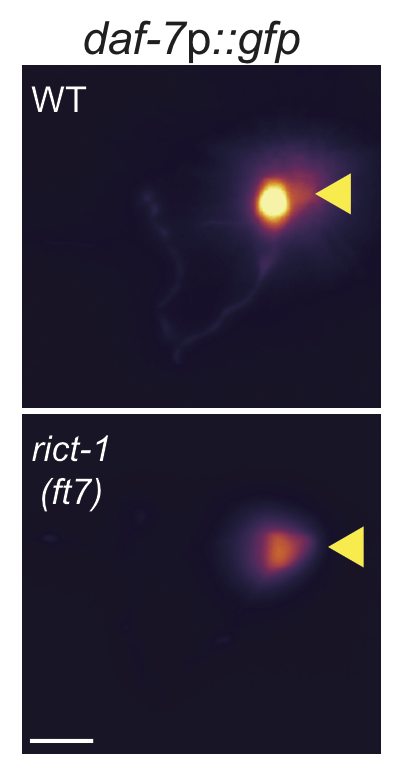
\includegraphics[width=5.54in]{/Users/mikeod/git/projects/dauergut/figures/2A_daf7GFP}

\begin{Shaded}
\begin{Highlighting}[]
\NormalTok{p}
\end{Highlighting}
\end{Shaded}

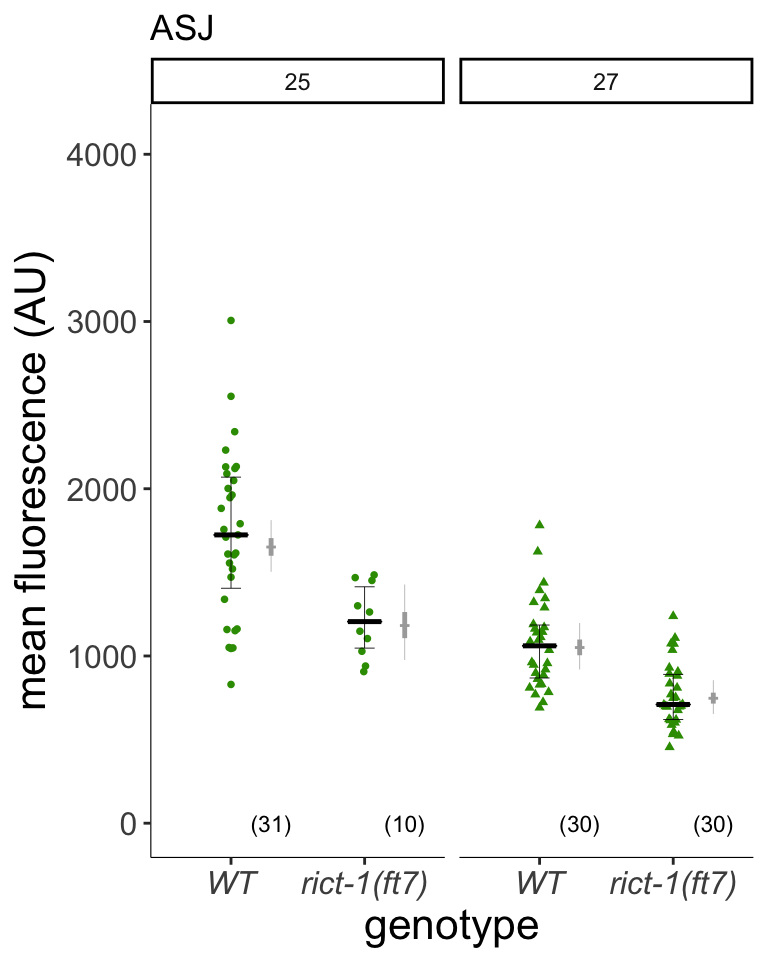
\includegraphics{Figure_2_files/figure-latex/unnamed-chunk-2-1.pdf}

\textbf{Figure 2A}\\
Intesinal \emph{rict-1} regulates daf7GFP levels in ASI neurons.
Daf-7::GFP fluorescence quantification shows decreased expression in
\emph{rict-1} mutants. Intestinal expression of \emph{rict-1} using the
intestinal \emph{ges-1} promoter rescues daf-7::GFP expression. (Left)
Representative images of \emph{daf-7p::gfp} expression in one of the
bilateral ASI neurons in animals of the indicated genotypes. Yellow
filled and open arrowheads indicate ASI and ASJ soma, respectively.
Anterior is at left. Scale bar: 5 μm. (Right) Quantification of
daf-7p::gfp expression in ASI (A) and daf-28p::gfp expression in ASI and
ASJ (D). Each dot is the mean fluorescence intensity in a single animal
(2 neurons per animal); numbers in parentheses below indicate the number
of animals examined in 3 independent experiments. Horizontal thick bar
indicates median. Error bars are quartiles. Light gray thin and thick
vertical bars at right indicate Bayesian 95\% and 75\% credible
intervals, respectively. {\texttt{**}} and {\texttt{***}} - different
from wild-type at P\textless{}0.01 and P\textless{}0.001, respectively;
{\texttt{***}} - different from rict-1(ft7) at P\textless{}0.001 (ANOVA
with Dunnett-type multivariate-t post-hoc adjustment). P-values of
differences in means relative to wild-type and corresponding mutant
animals are indicated in black and red, respectively.

\begin{Shaded}
\begin{Highlighting}[]
\KeywordTok{library}\NormalTok{(sjPlot)}
\KeywordTok{sjt.lm}\NormalTok{(linmod, }\DataTypeTok{depvar.labels =} \StringTok{"log(mean GFP intensity) (AU)"}\NormalTok{, }\DataTypeTok{show.se =} \OtherTok{TRUE}\NormalTok{, }\DataTypeTok{show.fstat =} \OtherTok{TRUE}\NormalTok{)}
\end{Highlighting}
\end{Shaded}

~

~

log(mean GFP intensity) (AU)

~

~

B

CI

std. Error

p

(Intercept)

~

3.44

3.41~--~3.48

0.02

\textless{}.001

genotype

mg360

~

-0.34

-0.41~--~-0.28

0.03

\textless{}.001

ft7

~

-0.17

-0.22~--~-0.12

0.03

\textless{}.001

ft7\_ges1resc

~

-0.00

-0.07~--~0.07

0.03

.966

ft7\_ifb2resc

~

-0.08

-0.15~--~-0.02

0.03

.017

ft7\_gpa4resc

~

-0.16

-0.23~--~-0.09

0.04

\textless{}.001

Observations

~

262

R2 / adj. R2

~

.345 / .332

F-statistics

~

26.954***

\begin{Shaded}
\begin{Highlighting}[]
\NormalTok{knitr}\OperatorTok{::}\KeywordTok{kable}\NormalTok{(contrasts, }\DataTypeTok{caption=}\StringTok{"Pairwise comparisons from ANOVA (Dunnett)"}\NormalTok{)}
\end{Highlighting}
\end{Shaded}

\begin{longtable}[]{@{}lrrrrrl@{}}
\caption{Pairwise comparisons from ANOVA (Dunnett)}\tabularnewline
\toprule
contrast & estimate & SE & df & t.ratio & p.value &
prange\tabularnewline
\midrule
\endfirsthead
\toprule
contrast & estimate & SE & df & t.ratio & p.value &
prange\tabularnewline
\midrule
\endhead
N2 - mg360 & 0.3444142 & 0.0335336 & 256 & 10.2707328 & 0.0000000 &
***\tabularnewline
N2 - ft7 & 0.1713309 & 0.0252778 & 256 & 6.7779166 & 0.0000000 &
***\tabularnewline
N2 - ft7\_ges1resc & 0.0014747 & 0.0348484 & 256 & 0.0423173 & 1.0000000
& p\textasciitilde{}1\tabularnewline
N2 - ft7\_ifb2resc & 0.0829684 & 0.0343846 & 256 & 2.4129517 & 0.1500418
& p\textasciitilde{}0.15\tabularnewline
N2 - ft7\_gpa4resc & 0.1642824 & 0.0358656 & 256 & 4.5804970 & 0.0001020
& ***\tabularnewline
mg360 - ft7 & -0.1730833 & 0.0336587 & 256 & -5.1423072 & 0.0000083 &
***\tabularnewline
mg360 - ft7\_ges1resc & -0.3429395 & 0.0413322 & 256 & -8.2971489 &
0.0000000 & ***\tabularnewline
mg360 - ft7\_ifb2resc & -0.2614458 & 0.0409419 & 256 & -6.3857752 &
0.0000000 & ***\tabularnewline
mg360 - ft7\_gpa4resc & -0.1801318 & 0.0421934 & 256 & -4.2691946 &
0.0003953 & ***\tabularnewline
ft7 - ft7\_ges1resc & -0.1698562 & 0.0349688 & 256 & -4.8573587 &
0.0000323 & ***\tabularnewline
ft7 - ft7\_ifb2resc & -0.0883625 & 0.0345066 & 256 & -2.5607400 &
0.1069585 & p\textasciitilde{}0.107\tabularnewline
ft7 - ft7\_gpa4resc & -0.0070485 & 0.0359826 & 256 & -0.1958866 &
0.9999577 & p\textasciitilde{}1\tabularnewline
ft7\_ges1resc - ft7\_ifb2resc & 0.0814937 & 0.0420256 & 256 & 1.9391429
& 0.3714490 & p\textasciitilde{}0.37\tabularnewline
ft7\_ges1resc - ft7\_gpa4resc & 0.1628077 & 0.0432458 & 256 & 3.7647094
& 0.0027464 & **\tabularnewline
ft7\_ifb2resc - ft7\_gpa4resc & 0.0813140 & 0.0428729 & 256 & 1.8966308
& 0.3970278 & p\textasciitilde{}0.4\tabularnewline
\bottomrule
\end{longtable}

\begin{Shaded}
\begin{Highlighting}[]
\NormalTok{knitr}\OperatorTok{::}\KeywordTok{kable}\NormalTok{(mixed[,}\KeywordTok{c}\NormalTok{(}\DecValTok{1}\OperatorTok{:}\DecValTok{6}\NormalTok{)], }\DataTypeTok{caption =} \StringTok{"Bayesian credible intervals"}\NormalTok{)}
\end{Highlighting}
\end{Shaded}

\begin{longtable}[]{@{}rrrrrl@{}}
\caption{Bayesian credible intervals}\tabularnewline
\toprule
mean & lower.CL & upper.CL & lower.25 & upper.75 &
genotype\tabularnewline
\midrule
\endfirsthead
\toprule
mean & lower.CL & upper.CL & lower.25 & upper.75 &
genotype\tabularnewline
\midrule
\endhead
2712.912 & 2361.302 & 3080.057 & 2602.961 & 2830.930 & N2\tabularnewline
1266.259 & 1050.407 & 1538.683 & 1187.433 & 1347.060 &
mg360\tabularnewline
1843.822 & 1585.181 & 2165.127 & 1752.443 & 1937.272 &
ft7\tabularnewline
2768.835 & 2271.144 & 3387.495 & 2596.101 & 2955.832 &
ft7\_ges1resc\tabularnewline
2252.374 & 1833.448 & 2795.261 & 2108.516 & 2401.470 &
ft7\_ifb2resc\tabularnewline
1866.109 & 1526.721 & 2311.558 & 1741.499 & 1994.483 &
ft7\_gpa4resc\tabularnewline
\bottomrule
\end{longtable}

\begin{Shaded}
\begin{Highlighting}[]
\NormalTok{p2}
\end{Highlighting}
\end{Shaded}

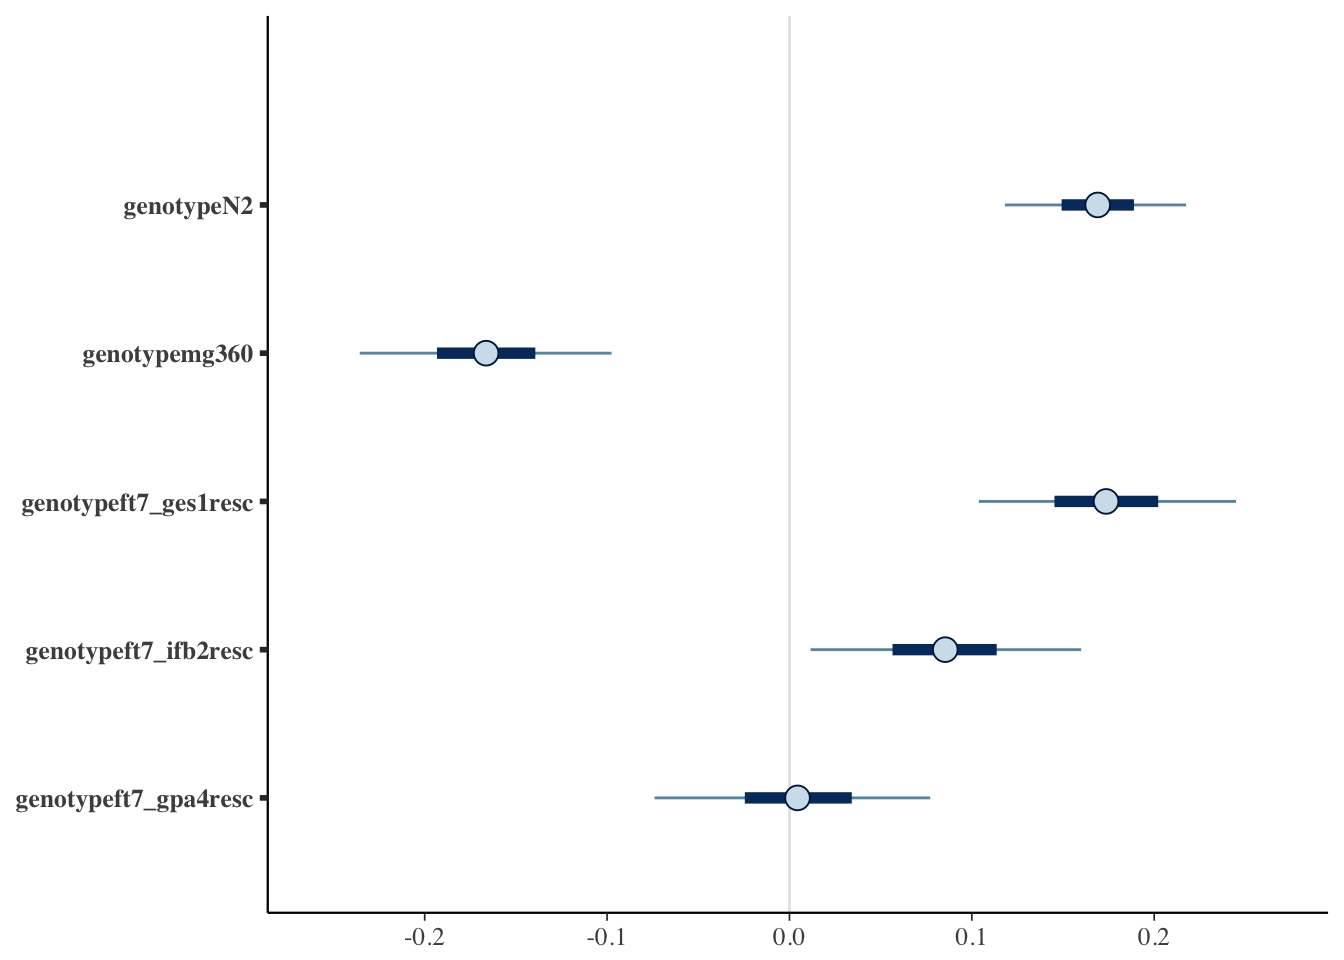
\includegraphics{Figure_2_files/figure-latex/2A daf-7 stats-1.pdf}

\subsection{2B}\label{b}

\begin{Shaded}
\begin{Highlighting}[]
\NormalTok{daf7FISH<-}\KeywordTok{read.csv}\NormalTok{(}\KeywordTok{file.path}\NormalTok{(pathname,}\StringTok{"extdata"}\NormalTok{,}\StringTok{"2B_daf7FISH_4frames.csv"}\NormalTok{)) }\OperatorTok
\StringTok{  }\KeywordTok{separate}\NormalTok{(Label, }\KeywordTok{c}\NormalTok{(}\StringTok{"method"}\NormalTok{,}\StringTok{"group"}\NormalTok{,}\StringTok{"sample"}\NormalTok{),}\DataTypeTok{sep =} \KeywordTok{c}\NormalTok{(}\StringTok{"-"}\NormalTok{), }\DataTypeTok{extra =} \StringTok{"drop"}\NormalTok{) }\OperatorTok
\StringTok{  }\KeywordTok{separate}\NormalTok{(sample, }\KeywordTok{c}\NormalTok{(}\StringTok{"sample"}\NormalTok{, }\StringTok{"type"}\NormalTok{),}\DataTypeTok{sep =}\StringTok{":"}\NormalTok{, }\DataTypeTok{extra =} \StringTok{"drop"}\NormalTok{) }\OperatorTok
\StringTok{  }\KeywordTok{mutate}\NormalTok{(}\DataTypeTok{genotype =} \KeywordTok{data.frame}\NormalTok{(}\KeywordTok{do.call}\NormalTok{(rbind, }\KeywordTok{strsplit}\NormalTok{(}\KeywordTok{as.vector}\NormalTok{(group), }\DataTypeTok{split =} \StringTok{"daf7_mRNA_L1_27d_"}\NormalTok{)))[,}\DecValTok{2}\NormalTok{],}
         \DataTypeTok{ID =} \KeywordTok{interaction}\NormalTok{(genotype, sample),}
         \DataTypeTok{genotype =} \KeywordTok{factor}\NormalTok{(genotype, }\DataTypeTok{levels =} \KeywordTok{c}\NormalTok{(}\StringTok{"N2"}\NormalTok{, }\StringTok{"ft7"}\NormalTok{, }\StringTok{"mg360"}\NormalTok{, }\StringTok{"mg360resc"}\NormalTok{)),}
         \DataTypeTok{group.id =}\NormalTok{ dplyr}\OperatorTok{::}\KeywordTok{case_when}\NormalTok{(}
\NormalTok{           genotype }\OperatorTok\StringTok{ }\KeywordTok{c}\NormalTok{(}\StringTok{"ft7"}\NormalTok{,}\StringTok{"mg360"}\NormalTok{) }\OperatorTok{~}\StringTok{ }\KeywordTok{as.character}\NormalTok{(}\StringTok{"mutant"}\NormalTok{),}
           \OtherTok{TRUE} \OperatorTok{~}\StringTok{ }\KeywordTok{as.character}\NormalTok{(genotype)))}

\CommentTok{#measured background fluorescence of each of 4 frames to normalize the sum projection of the neuron}
\CommentTok{#merge to add mean background value to each row:}
\NormalTok{background <-}\StringTok{ }\KeywordTok{filter}\NormalTok{(daf7FISH, type }\OperatorTok{==}\StringTok{ "background"}\NormalTok{) }\OperatorTok\StringTok{ }
\StringTok{  }\NormalTok{dplyr}\OperatorTok{::}\KeywordTok{select}\NormalTok{(ID, mean)}
\KeywordTok{colnames}\NormalTok{(background) <-}\StringTok{ }\KeywordTok{c}\NormalTok{(}\StringTok{"ID"}\NormalTok{, }\StringTok{"background"}\NormalTok{)}

\NormalTok{cells<-dplyr}\OperatorTok{::}\KeywordTok{filter}\NormalTok{(daf7FISH, type }\OperatorTok{==}\StringTok{ "cell"}\NormalTok{) }\OperatorTok\StringTok{ }\NormalTok{dplyr}\OperatorTok{::}\KeywordTok{select}\NormalTok{(ID, sample, mean, genotype, group.id)}
\KeywordTok{colnames}\NormalTok{(cells) <-}\StringTok{ }\KeywordTok{c}\NormalTok{(}\StringTok{"ID"}\NormalTok{, }\StringTok{"sample"}\NormalTok{, }\StringTok{"cell.mean"}\NormalTok{, }\StringTok{"genotype"}\NormalTok{,}\StringTok{"group.id"}\NormalTok{)}

\NormalTok{daf7FISH <-}\StringTok{ }\KeywordTok{merge}\NormalTok{(cells, background,}\DataTypeTok{by=}\StringTok{"ID"}\NormalTok{) }\OperatorTok
\StringTok{  }\KeywordTok{mutate}\NormalTok{(}\DataTypeTok{cell.norm =}\NormalTok{ cell.mean }\OperatorTok{-}\StringTok{ }\KeywordTok{mean}\NormalTok{(background),}
         \DataTypeTok{cell.diffnorm =}\NormalTok{ cell.mean }\OperatorTok{-}\StringTok{ }\NormalTok{background,}
         \DataTypeTok{cell.ratioNorm =}\NormalTok{ cell.mean }\OperatorTok{/}\StringTok{ }\NormalTok{background)}

\CommentTok{#simple lm}
\NormalTok{lm<-}\KeywordTok{lm}\NormalTok{(}\DataTypeTok{data=}\NormalTok{daf7FISH, }\DataTypeTok{formula=}\NormalTok{cell.norm}\OperatorTok{~}\NormalTok{genotype)}
\CommentTok{#check for outliers}
\NormalTok{daf7FISH <-}\StringTok{ }\NormalTok{dauergut}\OperatorTok{::}\KeywordTok{flag_outliers}\NormalTok{(lm, daf7FISH, }\DataTypeTok{threshold =} \DecValTok{4}\NormalTok{, }\DataTypeTok{noplot =} \OtherTok{TRUE}\NormalTok{)}

\NormalTok{lm.}\DecValTok{0}\NormalTok{<-}\KeywordTok{lm}\NormalTok{(}\DataTypeTok{data=}\NormalTok{daf7FISH[daf7FISH}\OperatorTok{$}\NormalTok{outlier.status }\OperatorTok{==}\StringTok{ }\OtherTok{FALSE}\NormalTok{,], }\DataTypeTok{formula=}\NormalTok{cell.norm}\OperatorTok{~}\DecValTok{1}\NormalTok{)}
\NormalTok{lm.}\DecValTok{1}\NormalTok{<-}\KeywordTok{lm}\NormalTok{(}\DataTypeTok{data=}\NormalTok{daf7FISH[daf7FISH}\OperatorTok{$}\NormalTok{outlier.status }\OperatorTok{==}\StringTok{ }\OtherTok{FALSE}\NormalTok{,], }\DataTypeTok{formula=}\NormalTok{cell.norm}\OperatorTok{~}\NormalTok{genotype)}
\CommentTok{#anova(lm.0, lm.1) p ~ 0.013}


\NormalTok{stanlm <-}\StringTok{ }\KeywordTok{stan_glm}\NormalTok{(cell.norm }\OperatorTok{~}\StringTok{ }\NormalTok{genotype, }\DataTypeTok{data =}\NormalTok{ daf7FISH[daf7FISH}\OperatorTok{$}\NormalTok{outlier.status }\OperatorTok{==}\StringTok{ }\OtherTok{FALSE}\NormalTok{,])}




\CommentTok{#plot daf7 FISH}
\NormalTok{strains <-}\StringTok{ }\KeywordTok{levels}\NormalTok{(daf7FISH}\OperatorTok{$}\NormalTok{genotype)}
\NormalTok{contrasts <-}\StringTok{ }\NormalTok{dauergut}\OperatorTok{::}\KeywordTok{dunnett_contrasts}\NormalTok{(lm.}\DecValTok{1}\NormalTok{,}\DataTypeTok{ref.index =} \DecValTok{1}\NormalTok{,}\StringTok{"genotype"}\NormalTok{)}
\NormalTok{mixed <-}\StringTok{ }\NormalTok{stanlm }\OperatorTok\StringTok{ }\NormalTok{dauergut}\OperatorTok{::}\KeywordTok{getStan_CIs}\NormalTok{()}
\NormalTok{rescue.test <-}\StringTok{ }\NormalTok{daf7FISH[daf7FISH}\OperatorTok{$}\NormalTok{outlier.status }\OperatorTok{==}\StringTok{ }\OtherTok{FALSE}\NormalTok{,] }\OperatorTok\StringTok{ }\KeywordTok{subset}\NormalTok{(genotype }\OperatorTok\StringTok{ }\KeywordTok{c}\NormalTok{(}\StringTok{"mg360"}\NormalTok{, }\StringTok{"mg360resc"}\NormalTok{)) }\OperatorTok\StringTok{ }\KeywordTok{t.test}\NormalTok{(cell.norm }\OperatorTok{~}\StringTok{ }\NormalTok{genotype)}
\NormalTok{rescue.p <-}\StringTok{ }\KeywordTok{data.frame}\NormalTok{(}\DataTypeTok{p.value =}\NormalTok{ rescue.test}\OperatorTok{$}\NormalTok{p.value) }\OperatorTok\StringTok{ }\NormalTok{dauergut}\OperatorTok{::}\KeywordTok{prange}\NormalTok{()}

\NormalTok{plot.contrasts <-}\StringTok{ }\KeywordTok{c}\NormalTok{(}\StringTok{""}\NormalTok{, contrasts}\OperatorTok{$}\NormalTok{prange[}\DecValTok{1}\OperatorTok{:}\DecValTok{2}\NormalTok{],}\StringTok{""}\NormalTok{)}
\NormalTok{plot.contrasts.}\DecValTok{2}\NormalTok{ <-}\StringTok{ }\KeywordTok{c}\NormalTok{(}\StringTok{""}\NormalTok{, }\StringTok{""}\NormalTok{, }\StringTok{""}\NormalTok{, rescue.p}\OperatorTok{$}\NormalTok{prange)}

\NormalTok{labels <-}\StringTok{ }\KeywordTok{c}\NormalTok{(}\StringTok{"WT"}\NormalTok{,}\StringTok{"rict-1(ft7)"}\NormalTok{,}\StringTok{"rict-1(mg360)"}\NormalTok{ ,}\StringTok{"rict-1(mg360); +ges1p::rict-1"}\NormalTok{) }\OperatorTok\StringTok{ }\NormalTok{stringr}\OperatorTok{::}\KeywordTok{str_wrap}\NormalTok{(}\DataTypeTok{width =} \DecValTok{10}\NormalTok{)}

\NormalTok{dauergut}\OperatorTok{::}\KeywordTok{plot_CIs}\NormalTok{(daf7FISH[daf7FISH}\OperatorTok{$}\NormalTok{outlier.status }\OperatorTok{==}\StringTok{ }\OtherTok{FALSE}\NormalTok{,], }\DataTypeTok{title =} \StringTok{"daf7 mRNA is reduced in rict-1 mutants"}\NormalTok{, }\DataTypeTok{plot.contrasts =}\NormalTok{ plot.contrasts, }\DataTypeTok{plot.contrasts.2 =}\NormalTok{ plot.contrasts.}\DecValTok{2}\NormalTok{, }\DataTypeTok{ypos =} \DecValTok{150}\NormalTok{, }\DataTypeTok{offset =} \DecValTok{0}\NormalTok{, }\DataTypeTok{type =} \StringTok{"expression"}\NormalTok{, }\DataTypeTok{labels =}\NormalTok{ labels)}
\end{Highlighting}
\end{Shaded}

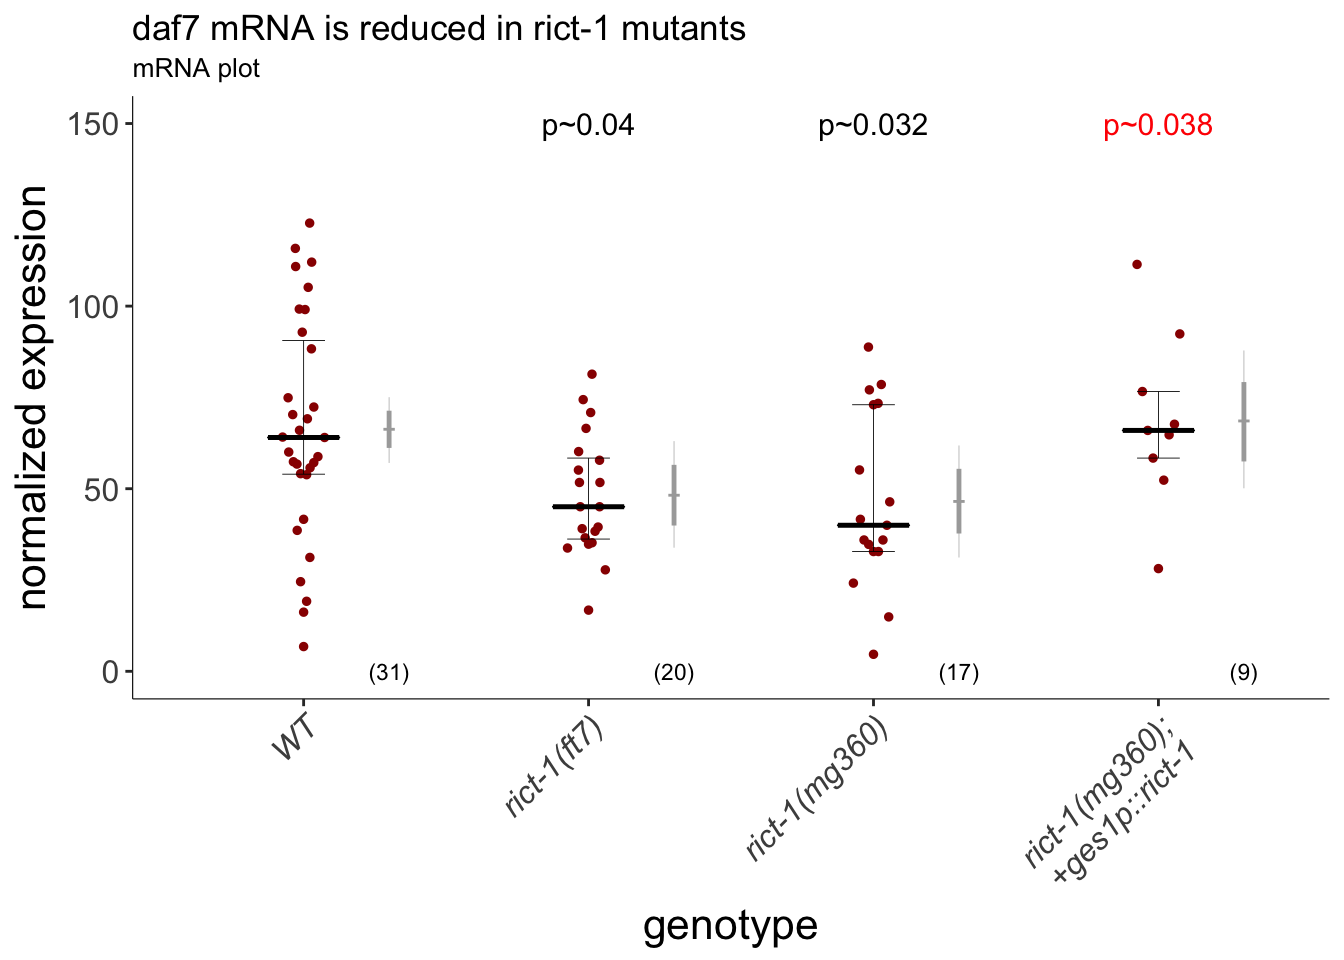
\includegraphics{Figure_2_files/figure-latex/daf7 FISH-1.pdf}

\textbf{Figure 2B} \emph{daf-7} mRNA is reduced in \emph{rict-1}
mutants. Intestinal expression of \emph{rict-1} using the intestinal
\emph{ges-1} promoter rescues \emph{daf-7} expression. Quantification of
\emph{daf-7} mRNA levels in ASI assessed via fluorescent in situ
hybridization. Expression was normalized by subtracting mean background
pixel values for each image. Each dot is the fluorescence intensity in a
single ASI neuron; numbers in parentheses below indicate the number of
neurons examined in 3 independent pooled experiments. Horizontal thick
bar indicates median. Error bars are quartiles. Light gray thin and
thick vertical bars at right indicate Bayesian 95\% and 75\% credible
intervals, respectively. P-values of differences relative to wild-type
and rict-1(mg360) animals are indicated in black and red, respectively.
For \emph{rict-1(mg360)} and \emph{rict-1(ft7)}, p\textasciitilde{}0.04
and p\textasciitilde{}0.032 compared to N2, respectively. For
\emph{ges-1} rescue, {p\textasciitilde{}0.038} compared to
\emph{rict-1(ft7)}. n=2 independent experiments, pooled data. 2 outlier
data points were removed in total. P-values of differences in means
relative to wild-type and corresponding mutant animals are indicated in
black and red, respectively.

\begin{Shaded}
\begin{Highlighting}[]
\KeywordTok{library}\NormalTok{(sjPlot)}
\KeywordTok{sjt.lm}\NormalTok{(lm.}\DecValTok{1}\NormalTok{, }\DataTypeTok{depvar.labels =} \StringTok{"mean mRNA levels (AU)"}\NormalTok{, }\DataTypeTok{show.se =} \OtherTok{TRUE}\NormalTok{, }\DataTypeTok{show.fstat =} \OtherTok{TRUE}\NormalTok{)}
\end{Highlighting}
\end{Shaded}

~

~

mean mRNA levels (AU)

~

~

B

CI

std. Error

p

(Intercept)

~

66.41

57.31~--~75.51

4.57

\textless{}.001

genotype

ft7

~

-18.33

-32.87~--~-3.80

7.29

.014

mg360

~

-19.95

-35.24~--~-4.65

7.67

.011

mg360resc

~

2.22

-16.97~--~21.41

9.63

.819

Observations

~

77

R2 / adj. R2

~

.136 / .100

F-statistics

~

3.826*

\begin{Shaded}
\begin{Highlighting}[]
\NormalTok{knitr}\OperatorTok{::}\KeywordTok{kable}\NormalTok{(contrasts, }\DataTypeTok{caption=}\StringTok{"Pairwise comparisons from ANOVA (Dunnett)"}\NormalTok{)}
\end{Highlighting}
\end{Shaded}

\begin{longtable}[]{@{}lrrrrrl@{}}
\caption{Pairwise comparisons from ANOVA (Dunnett)}\tabularnewline
\toprule
contrast & estimate & SE & df & t.ratio & p.value &
prange\tabularnewline
\midrule
\endfirsthead
\toprule
contrast & estimate & SE & df & t.ratio & p.value &
prange\tabularnewline
\midrule
\endhead
ft7 - N2 & -18.334597 & 7.293687 & 73 & -2.5137625 & 0.0401017 &
p\textasciitilde{}0.04\tabularnewline
mg360 - N2 & -19.946391 & 7.674908 & 73 & -2.5989094 & 0.0323168 &
p\textasciitilde{}0.032\tabularnewline
mg360resc - N2 & 2.216681 & 9.629102 & 73 & 0.2302064 & 0.9930297 &
p\textasciitilde{}1\tabularnewline
\bottomrule
\end{longtable}

\begin{Shaded}
\begin{Highlighting}[]
\NormalTok{knitr}\OperatorTok{::}\KeywordTok{kable}\NormalTok{(mixed[,}\KeywordTok{c}\NormalTok{(}\DecValTok{6}\NormalTok{,}\DecValTok{1}\OperatorTok{:}\DecValTok{5}\NormalTok{)], }\DataTypeTok{caption =} \StringTok{"Bayesian credible intervals"}\NormalTok{)}
\end{Highlighting}
\end{Shaded}

\begin{longtable}[]{@{}lrrrrr@{}}
\caption{Bayesian credible intervals}\tabularnewline
\toprule
genotype & mean & lower.CL & upper.CL & lower.25 &
upper.75\tabularnewline
\midrule
\endfirsthead
\toprule
genotype & mean & lower.CL & upper.CL & lower.25 &
upper.75\tabularnewline
\midrule
\endhead
N2 & 66.25145 & 57.35116 & 75.15967 & 63.12185 & 69.35324\tabularnewline
ft7 & 48.19804 & 33.30278 & 62.80688 & 43.17304 &
53.26688\tabularnewline
mg360 & 46.58205 & 31.82434 & 61.40551 & 41.44956 &
51.82490\tabularnewline
mg360resc & 68.67964 & 49.76890 & 88.20559 & 62.38462 &
74.87631\tabularnewline
\bottomrule
\end{longtable}

\subsection{2C}\label{c}

\begin{Shaded}
\begin{Highlighting}[]
\CommentTok{#days = as.factor(8:10) # days containing N2 and ft7 27º data}
\NormalTok{dates =}\StringTok{ }\KeywordTok{c}\NormalTok{(}\StringTok{"12_1_16"}\NormalTok{,  }\StringTok{"12_20_17"}\NormalTok{, }\StringTok{"12_21_17"}\NormalTok{, }\StringTok{"12_6_16"}\NormalTok{,  }\StringTok{"9_21_16"}\NormalTok{ )}
\NormalTok{strains =}\StringTok{ }\KeywordTok{c}\NormalTok{(}\StringTok{"N2"}\NormalTok{, }\StringTok{"ft7"}\NormalTok{, }\StringTok{"ft7exifb2"}\NormalTok{, }\StringTok{"ft7exgpa4"}\NormalTok{)}
\NormalTok{foods =}\StringTok{ "OP50"}
\NormalTok{d28<-}\KeywordTok{read.csv}\NormalTok{(}\StringTok{'extdata/2C_Daf28GFP_rescue.csv'}\NormalTok{) }\OperatorTok
\KeywordTok{separate}\NormalTok{(ID, }\KeywordTok{c}\NormalTok{(}\StringTok{"ID.A"}\NormalTok{, }\StringTok{"ID.B"}\NormalTok{), }\DataTypeTok{sep =} \StringTok{":"}\NormalTok{, }\DataTypeTok{extra =} \StringTok{"drop"}\NormalTok{) }\OperatorTok
\StringTok{  }\KeywordTok{subset}\NormalTok{(mean}\OperatorTok{!=}\DecValTok{4095} \OperatorTok{&}\StringTok{ }\NormalTok{food }\OperatorTok{==}\StringTok{ }\NormalTok{foods }\OperatorTok{&}\StringTok{ }\NormalTok{temp }\OperatorTok{==}\StringTok{ "27"} \OperatorTok{&}\StringTok{ }\NormalTok{genotype }\OperatorTok\StringTok{ }\NormalTok{strains }\OperatorTok{&}\StringTok{ }\NormalTok{pheromone }\OperatorTok{==}\StringTok{ }\DecValTok{0}\NormalTok{) }\OperatorTok
\StringTok{  }\KeywordTok{mutate}\NormalTok{(}\DataTypeTok{genotype =} \KeywordTok{factor}\NormalTok{(genotype, }\DataTypeTok{levels =}\NormalTok{ strains),}
         \DataTypeTok{genoID =} \KeywordTok{interaction}\NormalTok{(date,genotype, ID.A)}
\NormalTok{         )}

\NormalTok{df <-}\StringTok{ }\NormalTok{d28 }\OperatorTok\StringTok{ }\KeywordTok{group_by}\NormalTok{(neuron,date,genotype,genoID) }\OperatorTok\StringTok{ }
\StringTok{  }\KeywordTok{summarise}\NormalTok{(}\DataTypeTok{cell.norm =} \KeywordTok{mean}\NormalTok{(mean, }\DataTypeTok{na.rm =} \OtherTok{TRUE}\NormalTok{)) }\OperatorTok
\StringTok{  }\KeywordTok{data.frame}\NormalTok{() }\OperatorTok\StringTok{ }
\StringTok{  }\KeywordTok{mutate}\NormalTok{(}\DataTypeTok{group.id =} \KeywordTok{interaction}\NormalTok{(genotype, neuron),}
         \DataTypeTok{dataset =} \KeywordTok{case_when}\NormalTok{(}
\NormalTok{           date }\OperatorTok\StringTok{ }\KeywordTok{c}\NormalTok{(}\StringTok{"12_1_16"}\NormalTok{,}\StringTok{"12_6_16"}\NormalTok{,}\StringTok{"9_21_16"}\NormalTok{) }\OperatorTok{~}\StringTok{ "3C_3D"}\NormalTok{,}
\NormalTok{           date }\OperatorTok\StringTok{ }\KeywordTok{c}\NormalTok{(}\StringTok{"12_20_17"}\NormalTok{, }\StringTok{"12_21_17"}\NormalTok{) }\OperatorTok{~}\StringTok{ "_new"}
\NormalTok{         )) }\CommentTok{# take mean of each worm}
\end{Highlighting}
\end{Shaded}

\begin{Shaded}
\begin{Highlighting}[]
\NormalTok{day.means <-}\StringTok{ }\NormalTok{df }\OperatorTok
\StringTok{  }\KeywordTok{filter}\NormalTok{(genotype }\OperatorTok{==}\StringTok{ "ft7"}\NormalTok{) }\OperatorTok\StringTok{ }
\StringTok{  }\KeywordTok{group_by}\NormalTok{(date,neuron) }\OperatorTok
\StringTok{  }\KeywordTok{summarise}\NormalTok{(}\DataTypeTok{mean_ft7 =} \KeywordTok{mean}\NormalTok{(cell.norm)) }\OperatorTok\StringTok{ }\KeywordTok{data.frame}\NormalTok{()}

\CommentTok{#normalize to mean rict-1 mutant ASJ value per day}
\NormalTok{df }\OperatorTok\StringTok{ }\KeywordTok{mutate}\NormalTok{(}\DataTypeTok{cell.norm =} 
                 \KeywordTok{case_when}\NormalTok{(}
\NormalTok{                   neuron }\OperatorTok{==}\StringTok{ "ASI"} \OperatorTok{~}\StringTok{ }\KeywordTok{case_when}\NormalTok{(}
\NormalTok{                     date }\OperatorTok{==}\StringTok{ }\NormalTok{dates[}\DecValTok{1}\NormalTok{] }\OperatorTok{~}\StringTok{ }\NormalTok{(cell.norm }\OperatorTok{*}\StringTok{ }\NormalTok{day.means[}\DecValTok{2}\NormalTok{,}\DecValTok{3}\NormalTok{]) }\OperatorTok{/}\StringTok{ }\NormalTok{day.means[}\DecValTok{2}\NormalTok{,}\DecValTok{3}\NormalTok{],}
\NormalTok{                     date }\OperatorTok{==}\StringTok{ }\NormalTok{dates[}\DecValTok{2}\NormalTok{] }\OperatorTok{~}\StringTok{ }\NormalTok{(cell.norm }\OperatorTok{*}\StringTok{ }\NormalTok{day.means[}\DecValTok{2}\NormalTok{,}\DecValTok{3}\NormalTok{]) }\OperatorTok{/}\StringTok{ }\NormalTok{day.means[}\DecValTok{4}\NormalTok{,}\DecValTok{3}\NormalTok{],}
\NormalTok{                     date }\OperatorTok{==}\StringTok{ }\NormalTok{dates[}\DecValTok{3}\NormalTok{] }\OperatorTok{~}\StringTok{ }\NormalTok{(cell.norm }\OperatorTok{*}\StringTok{ }\NormalTok{day.means[}\DecValTok{2}\NormalTok{,}\DecValTok{3}\NormalTok{]) }\OperatorTok{/}\StringTok{ }\NormalTok{day.means[}\DecValTok{6}\NormalTok{,}\DecValTok{3}\NormalTok{],}
\NormalTok{                     date }\OperatorTok{==}\StringTok{ }\NormalTok{dates[}\DecValTok{4}\NormalTok{] }\OperatorTok{~}\StringTok{ }\NormalTok{(cell.norm }\OperatorTok{*}\StringTok{ }\NormalTok{day.means[}\DecValTok{2}\NormalTok{,}\DecValTok{3}\NormalTok{]) }\OperatorTok{/}\StringTok{ }\NormalTok{day.means[}\DecValTok{8}\NormalTok{,}\DecValTok{3}\NormalTok{],}
\NormalTok{                     date }\OperatorTok{==}\StringTok{ }\NormalTok{dates[}\DecValTok{5}\NormalTok{] }\OperatorTok{~}\StringTok{ }\NormalTok{(cell.norm }\OperatorTok{*}\StringTok{ }\NormalTok{day.means[}\DecValTok{2}\NormalTok{,}\DecValTok{3}\NormalTok{]) }\OperatorTok{/}\StringTok{ }\NormalTok{day.means[}\DecValTok{10}\NormalTok{,}\DecValTok{3}\NormalTok{]}
\NormalTok{                   ),}
\NormalTok{                   neuron }\OperatorTok{==}\StringTok{ "ASJ"} \OperatorTok{~}\StringTok{ }\KeywordTok{case_when}\NormalTok{(}
\NormalTok{                     date }\OperatorTok{==}\StringTok{ }\NormalTok{dates[}\DecValTok{1}\NormalTok{] }\OperatorTok{~}\StringTok{ }\NormalTok{cell.norm,}
\NormalTok{                     date }\OperatorTok{==}\StringTok{ }\NormalTok{dates[}\DecValTok{2}\NormalTok{] }\OperatorTok{~}\StringTok{ }\NormalTok{(cell.norm }\OperatorTok{*}\StringTok{ }\NormalTok{day.means[}\DecValTok{2}\NormalTok{,}\DecValTok{3}\NormalTok{]) }\OperatorTok{/}\StringTok{ }\NormalTok{day.means[}\DecValTok{4}\NormalTok{,}\DecValTok{3}\NormalTok{],}
\NormalTok{                     date }\OperatorTok{==}\StringTok{ }\NormalTok{dates[}\DecValTok{3}\NormalTok{] }\OperatorTok{~}\StringTok{ }\NormalTok{(cell.norm }\OperatorTok{*}\StringTok{ }\NormalTok{day.means[}\DecValTok{2}\NormalTok{,}\DecValTok{3}\NormalTok{]) }\OperatorTok{/}\StringTok{ }\NormalTok{day.means[}\DecValTok{6}\NormalTok{,}\DecValTok{3}\NormalTok{],}
\NormalTok{                     date }\OperatorTok{==}\StringTok{ }\NormalTok{dates[}\DecValTok{4}\NormalTok{] }\OperatorTok{~}\StringTok{ }\NormalTok{(cell.norm }\OperatorTok{*}\StringTok{ }\NormalTok{day.means[}\DecValTok{2}\NormalTok{,}\DecValTok{3}\NormalTok{]) }\OperatorTok{/}\StringTok{ }\NormalTok{day.means[}\DecValTok{8}\NormalTok{,}\DecValTok{3}\NormalTok{],}
\NormalTok{                     date }\OperatorTok{==}\StringTok{ }\NormalTok{dates[}\DecValTok{5}\NormalTok{] }\OperatorTok{~}\StringTok{ }\NormalTok{(cell.norm }\OperatorTok{*}\StringTok{ }\NormalTok{day.means[}\DecValTok{2}\NormalTok{,}\DecValTok{3}\NormalTok{]) }\OperatorTok{/}\StringTok{ }\NormalTok{day.means[}\DecValTok{10}\NormalTok{,}\DecValTok{3}\NormalTok{]}
\NormalTok{                   )}
\NormalTok{                 )}
\NormalTok{)}
  


\CommentTok{#fit simple linmod to est outliers:}
\NormalTok{log.tran<-lsmeans}\OperatorTok{::}\KeywordTok{make.tran}\NormalTok{(}\DataTypeTok{type=}\StringTok{"genlog"}\NormalTok{, }\DataTypeTok{param =} \KeywordTok{c}\NormalTok{(}\DecValTok{0}\NormalTok{,}\DecValTok{10}\NormalTok{)) }\CommentTok{#make log10 transformation}
\NormalTok{lm1 <-}\StringTok{ }\KeywordTok{with}\NormalTok{(log.tran, }\KeywordTok{lm}\NormalTok{(}\KeywordTok{linkfun}\NormalTok{(cell.norm) }\OperatorTok{~}\StringTok{ }\NormalTok{neuron }\OperatorTok{*}\StringTok{ }\NormalTok{genotype, }\DataTypeTok{data =}\NormalTok{ df))}
\NormalTok{df }\OperatorTok\StringTok{ }\KeywordTok{flag_outliers}\NormalTok{(}\DataTypeTok{lin.mod=}\NormalTok{lm1, }\DataTypeTok{threshold =} \DecValTok{4}\NormalTok{, }\DataTypeTok{df =}\NormalTok{ ., }\DataTypeTok{noplot=}\OtherTok{TRUE}\NormalTok{)}

\CommentTok{# linear MM}
\NormalTok{lm <-}\StringTok{ }\KeywordTok{with}\NormalTok{(log.tran, }\KeywordTok{lm}\NormalTok{(}\KeywordTok{linkfun}\NormalTok{(cell.norm) }\OperatorTok{~}\StringTok{ }\NormalTok{neuron }\OperatorTok{*}\StringTok{ }\NormalTok{genotype, }\DataTypeTok{data =}\NormalTok{ df[df}\OperatorTok{$}\NormalTok{outlier.status}\OperatorTok{==}\OtherTok{FALSE}\NormalTok{,]))}
\NormalTok{stanlmer <-}\StringTok{ }\KeywordTok{with}\NormalTok{(log.tran, }\KeywordTok{stan_lmer}\NormalTok{(}\KeywordTok{linkfun}\NormalTok{(cell.norm) }\OperatorTok{~}\StringTok{ }\DecValTok{1} \OperatorTok{+}\StringTok{ }\NormalTok{group.id }\OperatorTok{+}\StringTok{ }\NormalTok{(}\DecValTok{1}\OperatorTok{|}\NormalTok{date) }\OperatorTok{+}\StringTok{ }\NormalTok{(}\DecValTok{1}\OperatorTok{:}\NormalTok{group.id}\OperatorTok{:}\NormalTok{date), }\DataTypeTok{data =}\NormalTok{ df[df}\OperatorTok{$}\NormalTok{outlier.status}\OperatorTok{==}\OtherTok{FALSE}\NormalTok{,]))}


\NormalTok{contrasts<-}\KeywordTok{summary}\NormalTok{(lsmeans}\OperatorTok{::}\KeywordTok{lsmeans}\NormalTok{(lm, pairwise }\OperatorTok{~}\StringTok{ }\NormalTok{genotype }\OperatorTok{|}\StringTok{ }\NormalTok{neuron)}\OperatorTok{$}\NormalTok{contrasts) }\OperatorTok\StringTok{ }\NormalTok{dauergut}\OperatorTok{::}\KeywordTok{prange}\NormalTok{()}
\NormalTok{mixed <-}\StringTok{ }\NormalTok{stanlmer }\OperatorTok\StringTok{ }\KeywordTok{getStan_CIs}\NormalTok{(}\DataTypeTok{type =} \StringTok{"log"}\NormalTok{, }\DataTypeTok{group =} \StringTok{"neuron"}\NormalTok{, }\DataTypeTok{base =} \DecValTok{10}\NormalTok{, }\DataTypeTok{compare_gt =} \OtherTok{TRUE}\NormalTok{) }\OperatorTok\StringTok{ }
\StringTok{  }\KeywordTok{mutate}\NormalTok{(}\DataTypeTok{x.pos =} \KeywordTok{rep}\NormalTok{(}\KeywordTok{c}\NormalTok{(}\FloatTok{1.3}\NormalTok{,}\FloatTok{2.3}\NormalTok{,}\FloatTok{3.3}\NormalTok{,}\FloatTok{4.3}\NormalTok{),}\DecValTok{2}\NormalTok{))}
\NormalTok{plot.contrasts<-}\KeywordTok{c}\NormalTok{(}\StringTok{""}\NormalTok{,contrasts}\OperatorTok{$}\NormalTok{prange[}\DecValTok{1}\OperatorTok{:}\DecValTok{3}\NormalTok{],}
                  \StringTok{""}\NormalTok{,contrasts}\OperatorTok{$}\NormalTok{prange[}\DecValTok{7}\OperatorTok{:}\DecValTok{9}\NormalTok{])}
\NormalTok{plot.contrasts.}\DecValTok{2}\NormalTok{<-}\KeywordTok{c}\NormalTok{(}\StringTok{""}\NormalTok{,}\StringTok{""}\NormalTok{,contrasts}\OperatorTok{$}\NormalTok{prange[}\DecValTok{4}\OperatorTok{:}\DecValTok{5}\NormalTok{],}
                    \StringTok{""}\NormalTok{,}\StringTok{""}\NormalTok{,contrasts}\OperatorTok{$}\NormalTok{prange[}\DecValTok{10}\OperatorTok{:}\DecValTok{11}\NormalTok{])}

\NormalTok{labels <-}\StringTok{ }\KeywordTok{c}\NormalTok{(}\StringTok{"WT"}\NormalTok{,}
            \StringTok{"rict-1(ft7)"}\NormalTok{, }
            \StringTok{"rict-1(ft7); +ifb2p::rict-1"}\NormalTok{,}
            \StringTok{"rict-1(ft7); +gpa4p::rict-1"}\NormalTok{) }\OperatorTok\StringTok{ }\NormalTok{stringr}\OperatorTok{::}\KeywordTok{str_wrap}\NormalTok{(}\DataTypeTok{width =} \DecValTok{10}\NormalTok{)}
\CommentTok{#plot}
\NormalTok{p <-}\StringTok{ }\NormalTok{df }\OperatorTok\StringTok{ }
\StringTok{  }\KeywordTok{ggplot}\NormalTok{(}\KeywordTok{aes}\NormalTok{(}\DataTypeTok{x=}\NormalTok{genotype, }\DataTypeTok{y =}\NormalTok{ cell.norm)) }\OperatorTok{+}
\StringTok{  }\KeywordTok{geom_quasirandom}\NormalTok{(}\KeywordTok{aes}\NormalTok{(}\DataTypeTok{y=}\NormalTok{cell.norm, }\DataTypeTok{pch =}\NormalTok{ dataset),}\DataTypeTok{cex=}\DecValTok{1}\NormalTok{,}\DataTypeTok{colour =} \StringTok{"#339900"}\NormalTok{,}
                           \DataTypeTok{width =} \FloatTok{0.075}\NormalTok{,}\DataTypeTok{size=}\FloatTok{0.3}\NormalTok{,}
                           \DataTypeTok{method =} \StringTok{'smiley'}\NormalTok{) }\OperatorTok{+}
\StringTok{  }\NormalTok{theme_my }\OperatorTok{+}
\StringTok{  }\KeywordTok{guides}\NormalTok{(}\DataTypeTok{pch=}\OtherTok{FALSE}\NormalTok{) }\OperatorTok{+}
\StringTok{  }\KeywordTok{list}\NormalTok{(dauergut}\OperatorTok{::}\KeywordTok{add.median}\NormalTok{(}\DataTypeTok{width =} \FloatTok{0.25}\NormalTok{), dauergut}\OperatorTok{::}\KeywordTok{add.quartiles}\NormalTok{()) }\OperatorTok{+}
\StringTok{  }\KeywordTok{labs}\NormalTok{(}\DataTypeTok{title =} \StringTok{"daf-28 is also reduced in rict-1 mutants"}\NormalTok{,}
           \DataTypeTok{y =} \StringTok{"mean GFP intensity"}\NormalTok{, }\DataTypeTok{x=}\StringTok{"genotype"}\NormalTok{) }\OperatorTok{+}
\StringTok{  }\KeywordTok{stat_summary}\NormalTok{(}\KeywordTok{aes}\NormalTok{(}\DataTypeTok{x=}\NormalTok{genotype, }\DataTypeTok{group =}\NormalTok{ genotype, }\DataTypeTok{y =} \DecValTok{3000}\NormalTok{), }\DataTypeTok{geom=}\StringTok{"text"}\NormalTok{, }\DataTypeTok{fun.data=}\NormalTok{box_annot,}
                    \DataTypeTok{label=}\NormalTok{plot.contrasts, }\DataTypeTok{size =} \DecValTok{4}\NormalTok{) }\OperatorTok{+}
\StringTok{  }\KeywordTok{stat_summary}\NormalTok{(}\KeywordTok{aes}\NormalTok{(}\DataTypeTok{x=}\NormalTok{genotype, }\DataTypeTok{group =}\NormalTok{ genotype, }\DataTypeTok{y =} \DecValTok{2800}\NormalTok{), }\DataTypeTok{geom=}\StringTok{"text"}\NormalTok{, }\DataTypeTok{fun.data=}\NormalTok{box_annot,}
                    \DataTypeTok{label=}\NormalTok{plot.contrasts.}\DecValTok{2}\NormalTok{, }\DataTypeTok{size =} \DecValTok{4}\NormalTok{, }\DataTypeTok{colour =} \StringTok{"red"}\NormalTok{) }\OperatorTok{+}
\StringTok{  }\KeywordTok{geom_errorbar}\NormalTok{(}\DataTypeTok{data=}\NormalTok{mixed, }\KeywordTok{aes}\NormalTok{(}\DataTypeTok{x=}\NormalTok{x.pos,}\DataTypeTok{y=}\NormalTok{mean, }\DataTypeTok{ymin=}\NormalTok{lower.CL, }\DataTypeTok{ymax=}\NormalTok{upper.CL),}
                     \DataTypeTok{width=}\DecValTok{0}\NormalTok{,}\DataTypeTok{colour =}\StringTok{"grey"}\NormalTok{, }\DataTypeTok{lwd=}\FloatTok{0.15}\NormalTok{) }\OperatorTok{+}
\StringTok{  }\KeywordTok{geom_errorbar}\NormalTok{(}\DataTypeTok{data=}\NormalTok{mixed, }\KeywordTok{aes}\NormalTok{(}\DataTypeTok{x=}\NormalTok{x.pos,}\DataTypeTok{y=}\NormalTok{mean, }\DataTypeTok{ymin =}\NormalTok{ lower.}\DecValTok{25}\NormalTok{, }\DataTypeTok{ymax =}\NormalTok{ upper.}\DecValTok{75}\NormalTok{),}
                     \DataTypeTok{width=}\DecValTok{0}\NormalTok{,}\DataTypeTok{colour =} \StringTok{"darkgrey"}\NormalTok{, }\DataTypeTok{lwd =} \FloatTok{0.15}\OperatorTok{+}\FloatTok{0.7}\NormalTok{) }\OperatorTok{+}
\StringTok{  }\KeywordTok{stat_summary}\NormalTok{(}\KeywordTok{aes}\NormalTok{(}\DataTypeTok{x=}\KeywordTok{as.numeric}\NormalTok{(}\KeywordTok{as.factor}\NormalTok{(genotype)) }\OperatorTok{+}\StringTok{ }\FloatTok{0.3}\NormalTok{,}\DataTypeTok{y=}\DecValTok{0}\NormalTok{,}\DataTypeTok{group =}\NormalTok{ genotype),}
                    \DataTypeTok{fun.data =}\NormalTok{ fun_length, }\DataTypeTok{geom =} \StringTok{"text"}\NormalTok{,}\DataTypeTok{size =} \DecValTok{4}\NormalTok{) }\OperatorTok{+}
\StringTok{  }\KeywordTok{facet_grid}\NormalTok{(.}\OperatorTok{~}\NormalTok{neuron) }\OperatorTok{+}\StringTok{ }
\StringTok{  }\KeywordTok{scale_x_discrete}\NormalTok{(}\DataTypeTok{labels =}\NormalTok{ labels) }\OperatorTok{+}
\StringTok{  }\KeywordTok{theme}\NormalTok{(}\DataTypeTok{strip.background =} \KeywordTok{element_blank}\NormalTok{(),}
        \DataTypeTok{strip.text =} \KeywordTok{element_text}\NormalTok{(}\DataTypeTok{size =} \DecValTok{16}\NormalTok{,}\DataTypeTok{face=}\StringTok{"bold"}\NormalTok{),}
        \DataTypeTok{axis.text.y =} \KeywordTok{element_text}\NormalTok{(}\DataTypeTok{size=}\DecValTok{12}\NormalTok{),}
        \DataTypeTok{axis.text.x =} \KeywordTok{element_text}\NormalTok{(}\DataTypeTok{size =} \DecValTok{12}\NormalTok{, }\DataTypeTok{face =} \StringTok{"italic"}\NormalTok{),}
        \DataTypeTok{axis.title =} \KeywordTok{element_text}\NormalTok{(}\DataTypeTok{size=}\DecValTok{16}\NormalTok{),}
        \DataTypeTok{panel.spacing.x=}\KeywordTok{unit}\NormalTok{(}\DecValTok{2}\NormalTok{,}\StringTok{"lines"}\NormalTok{))}

\CommentTok{#image of daf-28 GFP}
\NormalTok{img.path <-}\StringTok{ }\KeywordTok{file.path}\NormalTok{(pathname,}\StringTok{"figures"}\NormalTok{,}\StringTok{"2D_daf-28GFP.png"}\NormalTok{)}
\end{Highlighting}
\end{Shaded}

\begin{Shaded}
\begin{Highlighting}[]
\KeywordTok{include_graphics}\NormalTok{(img.path)                            }
\end{Highlighting}
\end{Shaded}

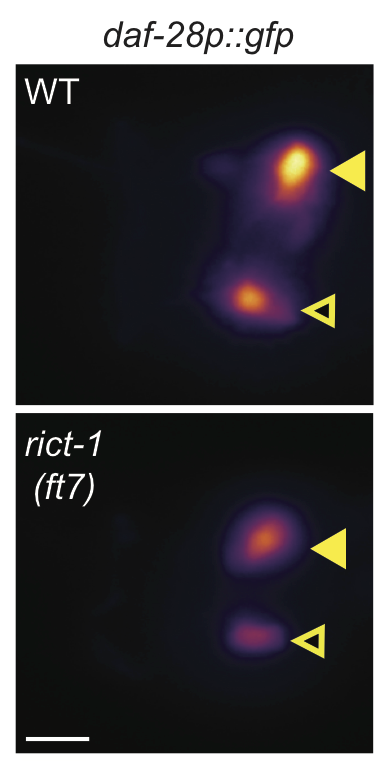
\includegraphics[width=5.42in]{/Users/mikeod/git/projects/dauergut/figures/2D_daf-28GFP}

\begin{Shaded}
\begin{Highlighting}[]
\NormalTok{p}
\end{Highlighting}
\end{Shaded}

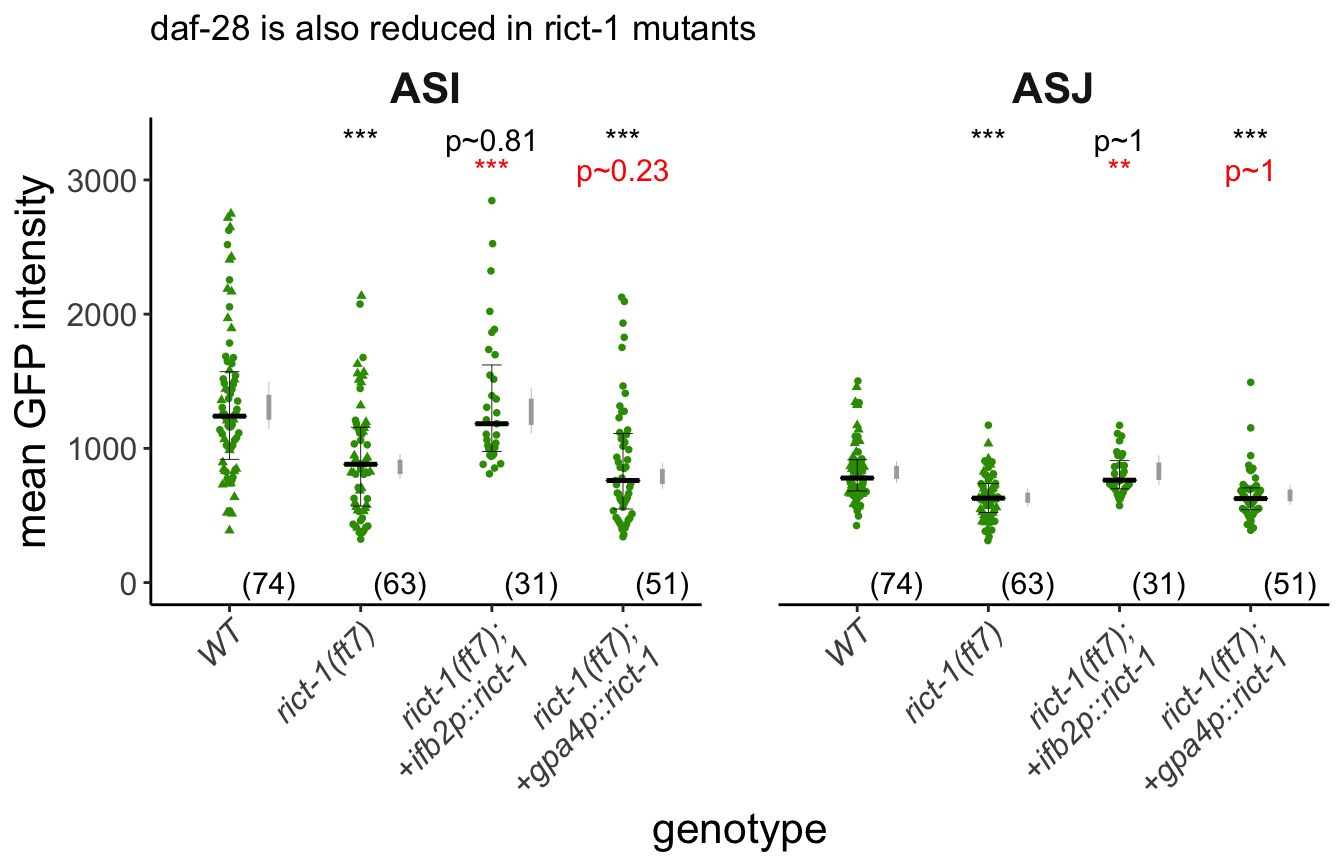
\includegraphics{Figure_2_files/figure-latex/unnamed-chunk-4-1.pdf}

\textbf{Figure 2C} (Left) Representative images of \emph{daf-28p::gfp}
expression in one of the bilateral and ASI and ASJ neurons in animals of
the indicated genotypes. Yellow filled and open arrowheads indicate ASI
and ASJ soma, respectively. Anterior is at left. Scale bar: 5 μm.
(Right) Quantification of \emph{daf-28p::gfp} expression in ASI and ASJ.
Each dot is the mean fluorescence intensity in a single animal (2
neurons per animal); numbers in parentheses below indicate the number of
animals examined in 3 independent experiments. Horizontal thick bar
indicates median. Error bars are quartiles. Light gray thin and thick
vertical bars at right indicate Bayesian 95\% and 75\% credible
intervals, respectively. {\texttt{**}} and {\texttt{***}} - different
from wild-type at P\textless{}0.01 and P\textless{}0.001, respectively;
(ANOVA with Tukey-type multivariate-t post-hoc adjustment).

\begin{Shaded}
\begin{Highlighting}[]
\KeywordTok{library}\NormalTok{(sjPlot)}
\KeywordTok{sjt.lm}\NormalTok{(lm, }\DataTypeTok{depvar.labels =} \StringTok{"log(mean GFP intensity) (AU)"}\NormalTok{, }\DataTypeTok{show.se =} \OtherTok{TRUE}\NormalTok{, }\DataTypeTok{show.fstat =} \OtherTok{TRUE}\NormalTok{)}
\end{Highlighting}
\end{Shaded}

~

~

log(mean GFP intensity) (AU)

~

~

B

CI

std. Error

p

(Intercept)

~

3.11

3.08~--~3.14

0.02

\textless{}.001

neuronASJ

~

-0.21

-0.25~--~-0.16

0.02

\textless{}.001

genotype

genotypeft7

~

-0.18

-0.23~--~-0.13

0.02

\textless{}.001

genotypeft7exifb2

~

-0.03

-0.09~--~0.03

0.03

.370

genotypeft7exgpa4

~

-0.23

-0.28~--~-0.18

0.03

\textless{}.001

neuronASJ:genotypeft7

~

0.07

0.00~--~0.14

0.03

.035

neuronASJ:genotypeft7exifb2

~

0.02

-0.06~--~0.10

0.04

.628

neuronASJ:genotypeft7exgpa4

~

0.12

0.05~--~0.19

0.04

\textless{}.001

Observations

~

417

R2 / adj. R2

~

.414 / .404

F-statistics

~

41.338***

\begin{Shaded}
\begin{Highlighting}[]
\NormalTok{knitr}\OperatorTok{::}\KeywordTok{kable}\NormalTok{(mixed[,}\KeywordTok{c}\NormalTok{(}\DecValTok{6}\NormalTok{,}\DecValTok{1}\OperatorTok{:}\DecValTok{5}\NormalTok{)], }\DataTypeTok{caption =} \StringTok{"Bayesian credible intervals"}\NormalTok{)}
\end{Highlighting}
\end{Shaded}

\begin{longtable}[]{@{}lrrrrr@{}}
\caption{Bayesian credible intervals}\tabularnewline
\toprule
genotype & mean & lower.CL & upper.CL & lower.25 &
upper.75\tabularnewline
\midrule
\endfirsthead
\toprule
genotype & mean & lower.CL & upper.CL & lower.25 &
upper.75\tabularnewline
\midrule
\endhead
N2 & 1295.1396 & 1132.6314 & 1470.6497 & 1247.1781 &
1346.2099\tabularnewline
ft7 & 856.8436 & 770.3667 & 954.7652 & 825.9815 &
889.4944\tabularnewline
ft7exifb2 & 1260.6311 & 1106.0919 & 1442.6340 & 1203.9105 &
1318.7281\tabularnewline
ft7exgpa4 & 784.1690 & 698.8073 & 884.8495 & 752.9071 &
816.0061\tabularnewline
N2 & 812.3631 & 735.8341 & 897.6822 & 785.5079 & 841.0360\tabularnewline
ft7 & 627.8258 & 568.3356 & 694.2214 & 604.9115 &
650.7897\tabularnewline
ft7exifb2 & 822.9861 & 722.4214 & 941.7833 & 786.5650 &
859.5863\tabularnewline
ft7exgpa4 & 645.2726 & 575.9766 & 722.6930 & 620.5738 &
671.3110\tabularnewline
\bottomrule
\end{longtable}

\begin{Shaded}
\begin{Highlighting}[]
\NormalTok{knitr}\OperatorTok{::}\KeywordTok{kable}\NormalTok{(contrasts, }\DataTypeTok{caption =} \StringTok{"pairwise comparisons (Tukey)"}\NormalTok{)}
\end{Highlighting}
\end{Shaded}

\begin{longtable}[]{@{}llrrrrrl@{}}
\caption{pairwise comparisons (Tukey)}\tabularnewline
\toprule
contrast & neuron & estimate & SE & df & t.ratio & p.value &
prange\tabularnewline
\midrule
\endfirsthead
\toprule
contrast & neuron & estimate & SE & df & t.ratio & p.value &
prange\tabularnewline
\midrule
\endhead
N2 - ft7 & ASI & 0.1812272 & 0.0240311 & 409 & 7.5413602 & 0.0000000 &
***\tabularnewline
N2 - ft7exifb2 & ASI & 0.0266916 & 0.0297459 & 409 & 0.8973202 &
0.8062379 & p\textasciitilde{}0.81\tabularnewline
N2 - ft7exgpa4 & ASI & 0.2331576 & 0.0260984 & 409 & 8.9337827 &
0.0000000 & ***\tabularnewline
ft7 - ft7exifb2 & ASI & -0.1545355 & 0.0307235 & 409 & -5.0298767 &
0.0000044 & ***\tabularnewline
ft7 - ft7exgpa4 & ASI & 0.0519304 & 0.0272074 & 409 & 1.9086898 &
0.2259441 & p\textasciitilde{}0.23\tabularnewline
ft7exifb2 - ft7exgpa4 & ASI & 0.2064660 & 0.0323662 & 409 & 6.3790679 &
0.0000000 & ***\tabularnewline
N2 - ft7 & ASJ & 0.1108181 & 0.0230904 & 409 & 4.7993066 & 0.0000133 &
***\tabularnewline
N2 - ft7exifb2 & ASJ & 0.0066176 & 0.0288175 & 409 & 0.2296397 &
0.9957282 & p\textasciitilde{}1\tabularnewline
N2 - ft7exgpa4 & ASJ & 0.1115180 & 0.0246586 & 409 & 4.5224807 &
0.0000473 & ***\tabularnewline
ft7 - ft7exifb2 & ASJ & -0.1042005 & 0.0295509 & 409 & -3.5261338 &
0.0026362 & **\tabularnewline
ft7 - ft7exgpa4 & ASJ & 0.0006998 & 0.0255119 & 409 & 0.0274322 &
0.9999926 & p\textasciitilde{}1\tabularnewline
ft7exifb2 - ft7exgpa4 & ASJ & 0.1049004 & 0.0307918 & 409 & 3.4067640 &
0.0040134 & **\tabularnewline
\bottomrule
\end{longtable}

\subsection{2D}\label{d}

\begin{Shaded}
\begin{Highlighting}[]
\NormalTok{strains<-}\KeywordTok{c}\NormalTok{(}\StringTok{"N2"}\NormalTok{, }\StringTok{"rict-1(mg360)"}\NormalTok{, }\StringTok{"rict-1(ft7)"}\NormalTok{)}
\CommentTok{#dates<-c("12_5_14", "12_19_14", "1_19_15","3_22_14", "2_25_14", "4_11_14")}
\NormalTok{dates<-}\KeywordTok{c}\NormalTok{(}\StringTok{"12_5_14"}\NormalTok{, }\StringTok{"12_19_14"}\NormalTok{,}\StringTok{"3_22_14"}\NormalTok{, }\StringTok{"2_25_14"}\NormalTok{, }\StringTok{"4_11_14"}\NormalTok{)}
\NormalTok{foods <-}\StringTok{ }\KeywordTok{c}\NormalTok{(}\StringTok{"OP50"}\NormalTok{, }\StringTok{"HB101"}\NormalTok{)}
\NormalTok{rict1.food<-}\KeywordTok{read.csv}\NormalTok{(}\KeywordTok{file.path}\NormalTok{(pathname, }\StringTok{"extdata"}\NormalTok{, }\StringTok{"1B_2D_rict-1_TORC2.csv"}\NormalTok{), }\DataTypeTok{header=}\OtherTok{TRUE}\NormalTok{) }\OperatorTok\StringTok{ }\KeywordTok{format_dauer}\NormalTok{(}\DataTypeTok{p.dauer =} \StringTok{"exclude"}\NormalTok{) }\OperatorTok
\StringTok{  }\NormalTok{dplyr}\OperatorTok{::}\KeywordTok{filter}\NormalTok{(day }\OperatorTok\StringTok{ }\NormalTok{dates) }\OperatorTok\StringTok{ }\KeywordTok{mutate}\NormalTok{(}\DataTypeTok{logit.p =}\NormalTok{ car}\OperatorTok{::}\KeywordTok{logit}\NormalTok{(pct, }\DataTypeTok{adjust=}\FloatTok{0.01}\NormalTok{), }
                                           \DataTypeTok{plate.ID =} \KeywordTok{interaction}\NormalTok{(food, plateID))}

\CommentTok{# rict1.food %>% ggplot(aes(x=food, y=pct)) + geom_boxplot() + stat_summary(aes(y=pct, group=day, colour = day), fun.y = mean, geom = "line") + facet_grid(.~genotype)}

\CommentTok{#lm}
\NormalTok{lm.add <-}\StringTok{ }\KeywordTok{lm}\NormalTok{(pct }\OperatorTok{~}\StringTok{ }\NormalTok{genotype }\OperatorTok{+}\StringTok{ }\NormalTok{food, }\DataTypeTok{data =}\NormalTok{ rict1.food)}
\NormalTok{lm.int <-}\StringTok{ }\KeywordTok{update}\NormalTok{(lm.add,.}\OperatorTok{~}\NormalTok{. }\OperatorTok{+}\StringTok{ }\NormalTok{genotype}\OperatorTok{*}\NormalTok{food)}
\CommentTok{#stan}
\NormalTok{rict.food.groups <-}\StringTok{ }\NormalTok{rict1.food }\OperatorTok\StringTok{ }\KeywordTok{mutate}\NormalTok{(}\DataTypeTok{group.id =} \KeywordTok{interaction}\NormalTok{(genotype, food))}
\NormalTok{stan.glmm <-}\StringTok{ }\KeywordTok{run_dauer_stan}\NormalTok{(}\DataTypeTok{df =}\NormalTok{ rict.food.groups, }\DataTypeTok{type=}\StringTok{"dauer-grouped"}\NormalTok{, }\DataTypeTok{group =} \StringTok{"food"}\NormalTok{, }\DataTypeTok{intercept =} \OtherTok{FALSE}\NormalTok{)}
\end{Highlighting}
\end{Shaded}

\begin{Shaded}
\begin{Highlighting}[]
\NormalTok{contrasts<-dauergut}\OperatorTok{::}\KeywordTok{dunnett_contrasts}\NormalTok{(lm.int, }\DataTypeTok{ref.index =} \DecValTok{1}\NormalTok{, }\DataTypeTok{factor =} \StringTok{"genotype"}\NormalTok{, }\DataTypeTok{interaction =} \StringTok{"food"}\NormalTok{)}
\NormalTok{mixed<-dauergut}\OperatorTok{::}\KeywordTok{getStan_CIs}\NormalTok{(stan.glmm, }\DataTypeTok{type=}\StringTok{"dauer"}\NormalTok{, }\DataTypeTok{group =} \StringTok{"food"}\NormalTok{, }\DataTypeTok{intercept =} \OtherTok{FALSE}\NormalTok{)}

\NormalTok{plot.contrasts <-}\StringTok{ }\KeywordTok{c}\NormalTok{(}\StringTok{""}\NormalTok{,contrasts}\OperatorTok{$}\NormalTok{interaction}\OperatorTok{$}\NormalTok{prange[}\DecValTok{1}\NormalTok{], }\StringTok{""}\NormalTok{, contrasts}\OperatorTok{$}\NormalTok{interaction}\OperatorTok{$}\NormalTok{prange[}\DecValTok{2}\NormalTok{], }\StringTok{""}\NormalTok{, contrasts}\OperatorTok{$}\NormalTok{interaction}\OperatorTok{$}\NormalTok{prange[}\DecValTok{3}\NormalTok{])}
\NormalTok{plot.contrasts.interaction <-}\StringTok{ }\KeywordTok{summary}\NormalTok{(lm.int)}\OperatorTok{$}\NormalTok{coefficients[,}\DecValTok{4}\NormalTok{][}\DecValTok{5}\OperatorTok{:}\DecValTok{6}\NormalTok{] }\OperatorTok\StringTok{ }\KeywordTok{data.frame}\NormalTok{() }\OperatorTok\StringTok{ }\KeywordTok{mutate}\NormalTok{(}\DataTypeTok{p.value =} \KeywordTok{c}\NormalTok{(.[[}\DecValTok{1}\NormalTok{]],.[[}\DecValTok{2}\NormalTok{]]), }\DataTypeTok{genotype =}\NormalTok{ strains[}\DecValTok{2}\OperatorTok{:}\DecValTok{3}\NormalTok{]) }\OperatorTok\StringTok{ }\NormalTok{dauergut}\OperatorTok{::}\KeywordTok{prange}\NormalTok{()}

\NormalTok{index<-}\KeywordTok{rep}\NormalTok{(}\KeywordTok{seq_len}\NormalTok{(}\KeywordTok{length}\NormalTok{(strains)), }\DataTypeTok{each =} \DecValTok{2}\NormalTok{)}

\NormalTok{plot.contrasts.H0 <-}\StringTok{ }\KeywordTok{data.frame}\NormalTok{(}\KeywordTok{cbind}\NormalTok{(}\DataTypeTok{food =}\NormalTok{ foods, }\DataTypeTok{genotype =}\NormalTok{ strains[index])) }\OperatorTok
\StringTok{  }\KeywordTok{mutate}\NormalTok{(}\DataTypeTok{prange =}\NormalTok{ plot.contrasts)}

\NormalTok{(p<-}\KeywordTok{ggplot}\NormalTok{(rict1.food, }\KeywordTok{aes}\NormalTok{(}\DataTypeTok{x=}\NormalTok{food)) }\OperatorTok{+}
\StringTok{  }\KeywordTok{stat_summary}\NormalTok{(}\KeywordTok{aes}\NormalTok{(}\DataTypeTok{y=}\NormalTok{pct, }\DataTypeTok{group=}\NormalTok{day), }\DataTypeTok{colour =} \StringTok{"black"}\NormalTok{, }\DataTypeTok{fun.y =}\NormalTok{ mean, }\DataTypeTok{geom =} \StringTok{"line"}\NormalTok{, }\DataTypeTok{alpha =} \FloatTok{0.2}\NormalTok{, }\DataTypeTok{linetype =} \DecValTok{2}\NormalTok{) }\OperatorTok{+}
\StringTok{  }\KeywordTok{add.median.dauer}\NormalTok{() }\OperatorTok{+}
\StringTok{  }\KeywordTok{add.Bayes.CI}\NormalTok{() }\OperatorTok{+}
\StringTok{  }\KeywordTok{geom_dotplot}\NormalTok{(}\KeywordTok{aes}\NormalTok{(}\DataTypeTok{y=}\NormalTok{pct, }\DataTypeTok{colour =}\NormalTok{ food, }\DataTypeTok{fill=}\NormalTok{food),}\DataTypeTok{binwidth=}\NormalTok{.}\DecValTok{015}\NormalTok{, }\DataTypeTok{binaxis=}\StringTok{"y"}\NormalTok{, }\DataTypeTok{position=}\StringTok{"dodge"}\NormalTok{, }\DataTypeTok{stackdir=}\StringTok{"center"}\NormalTok{, }\DataTypeTok{size =}\NormalTok{.}\DecValTok{3}\NormalTok{) }\OperatorTok{+}
\StringTok{    }\CommentTok{#geom_point(aes(y=pct,colour = food), size = 0.7, alpha = 0.75) +}
\StringTok{  }\KeywordTok{labs}\NormalTok{(}\DataTypeTok{title =} \StringTok{"rict-1 mutants are deficient in food suppression"}\NormalTok{,}
           \DataTypeTok{y =} \StringTok{"proportion dauer"}\NormalTok{,}
           \DataTypeTok{x =} \StringTok{"food"}\NormalTok{) }\OperatorTok{+}
\StringTok{  }\KeywordTok{facet_grid}\NormalTok{(.}\OperatorTok{~}\NormalTok{genotype, }\DataTypeTok{switch=}\StringTok{"both"}\NormalTok{) }\OperatorTok{+}
\StringTok{  }\KeywordTok{scale_colour_manual}\NormalTok{(}\DataTypeTok{values =} \KeywordTok{c}\NormalTok{(}\StringTok{"black"}\NormalTok{, }\StringTok{"#FF9933"}\NormalTok{)) }\OperatorTok{+}
\StringTok{    }\KeywordTok{scale_fill_manual}\NormalTok{(}\DataTypeTok{values =} \KeywordTok{c}\NormalTok{(}\StringTok{"black"}\NormalTok{, }\StringTok{"#FF9933"}\NormalTok{)) }\OperatorTok{+}
\StringTok{      }\KeywordTok{scale_y_continuous}\NormalTok{(}\DataTypeTok{breaks=}\KeywordTok{c}\NormalTok{(}\DecValTok{0}\NormalTok{,}\FloatTok{0.25}\NormalTok{,}\FloatTok{0.5}\NormalTok{,}\FloatTok{0.75}\NormalTok{, }\FloatTok{1.0}\NormalTok{)) }\OperatorTok{+}
\StringTok{      }\KeywordTok{scale_x_discrete}\NormalTok{(}\DataTypeTok{labels=}\ControlFlowTok{function}\NormalTok{(x) }\KeywordTok{sub}\NormalTok{(}\StringTok{" "}\NormalTok{,}\StringTok{"}\CharTok{\textbackslash{}n}\StringTok{"}\NormalTok{,x,}\DataTypeTok{fixed=}\OtherTok{TRUE}\NormalTok{)) }\OperatorTok{+}
\StringTok{  }\KeywordTok{geom_text}\NormalTok{(}\DataTypeTok{data =}\NormalTok{ plot.contrasts.H0, }\KeywordTok{aes}\NormalTok{(}\DataTypeTok{x=}\DecValTok{2}\NormalTok{, }\DataTypeTok{label =}\NormalTok{ prange, }\DataTypeTok{y =} \FloatTok{1.075}\NormalTok{, }\DataTypeTok{group =} \OtherTok{NULL}\NormalTok{), }\DataTypeTok{size =} \DecValTok{4}\NormalTok{) }\OperatorTok{+}
\StringTok{    }\KeywordTok{stat_summary}\NormalTok{(}\KeywordTok{aes}\NormalTok{(}\DataTypeTok{x=}\KeywordTok{as.numeric}\NormalTok{(}\KeywordTok{as.factor}\NormalTok{(food)) }\OperatorTok{+}\StringTok{ }\FloatTok{0.3}\NormalTok{, }\DataTypeTok{y=}\OperatorTok{-}\FloatTok{0.05}\NormalTok{),}
                   \DataTypeTok{fun.data =}\NormalTok{ fun_length, }\DataTypeTok{geom =} \StringTok{"text"}\NormalTok{, }\DataTypeTok{size =} \DecValTok{3}\NormalTok{) }\OperatorTok{+}
\StringTok{  }\KeywordTok{theme_classic}\NormalTok{() }\OperatorTok{+}\StringTok{ }
\StringTok{    }\KeywordTok{theme}\NormalTok{(}\DataTypeTok{strip.text.x =} \KeywordTok{element_text}\NormalTok{(}\DataTypeTok{size =} \DecValTok{12}\NormalTok{, }\DataTypeTok{face=}\StringTok{"italic"}\NormalTok{),}
      \DataTypeTok{axis.text.x =} \KeywordTok{element_blank}\NormalTok{(),}
          \DataTypeTok{axis.text.y =} \KeywordTok{element_text}\NormalTok{(}\DataTypeTok{size =} \DecValTok{12}\NormalTok{),}
          \DataTypeTok{axis.line =} \KeywordTok{element_line}\NormalTok{(}\DataTypeTok{size=}\FloatTok{0.2}\NormalTok{),}
          \DataTypeTok{axis.title =} \KeywordTok{element_text}\NormalTok{(}\DataTypeTok{size=}\DecValTok{16}\NormalTok{)))}
\end{Highlighting}
\end{Shaded}

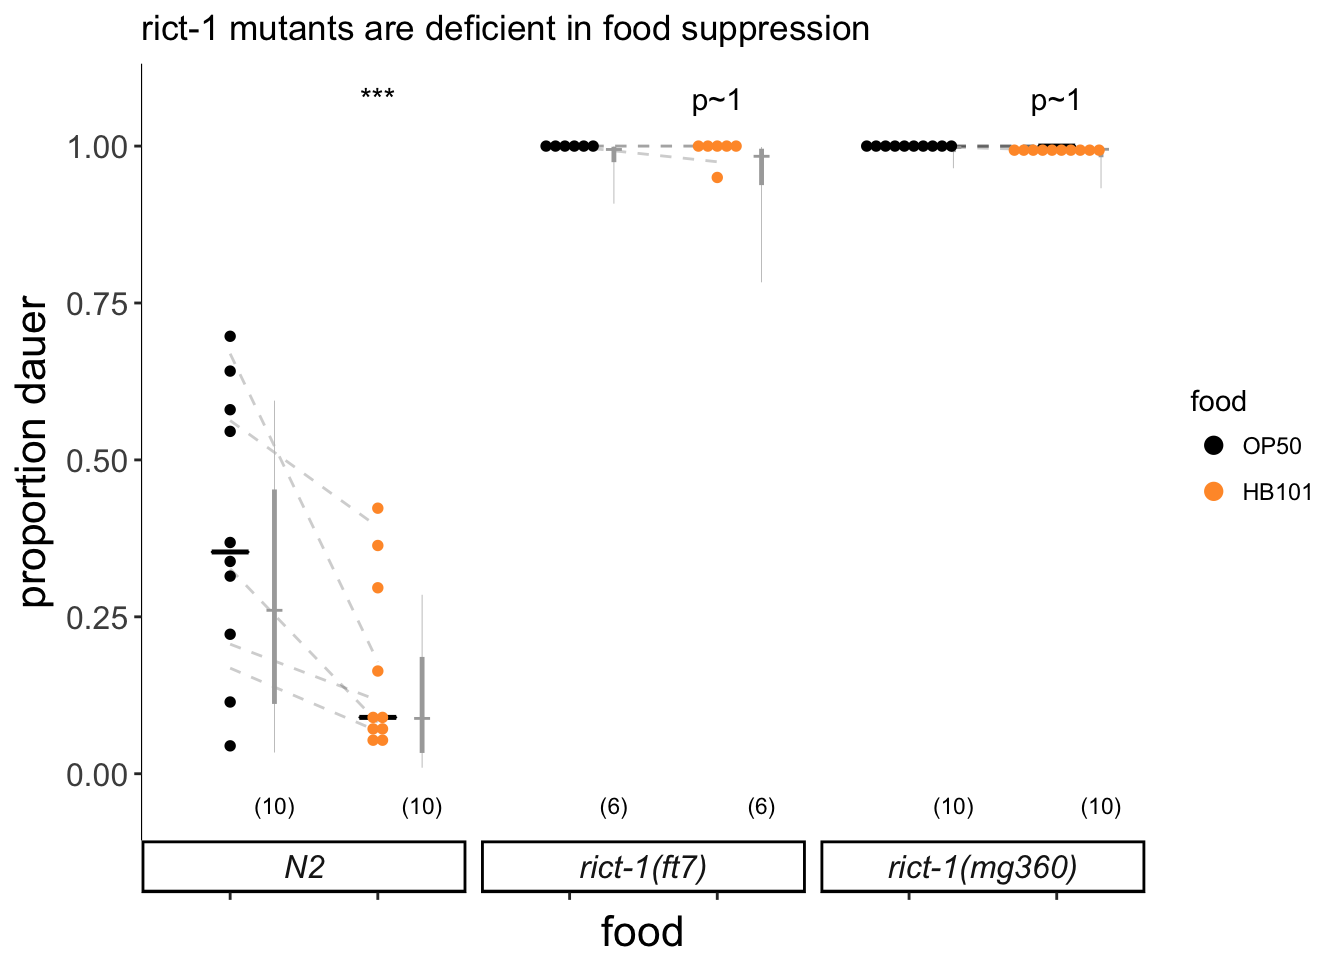
\includegraphics{Figure_2_files/figure-latex/rict-1 food plot-1.pdf}

\textbf{Figure 2D}\\
\emph{rict-1} mutants are deficient in food suppression of dauer
formation. Dauers formed by wild-type and rict-1 mutants on OP50 or
HB101 at 27°C. Each black dot indicates the average number of dauers
formed in a single assay. Horizontal black bar indicates median. Light
gray thin and thick vertical bars at right indicate Bayesian 95\% and
75\% credible intervals, respectively. Numbers in parentheses below
indicate the number of independent experiments with at least 19 animals
scored in each. Dashed lines indicate mean change in dauer formation per
experimental day. P-values are with respect to growth on OP50;
\texttt{***} - different from growth on OP50 at P\textless{}0.001
{[}two-factor ANOVA with F(5.21) with 2 Df, P=0.0092 for genotype*food
interaction, Tukey-type multivariate-t post-hoc adjustment{]}.

\begin{Shaded}
\begin{Highlighting}[]
\KeywordTok{library}\NormalTok{(sjPlot)}
\KeywordTok{sjt.lm}\NormalTok{(lm.int, }\DataTypeTok{depvar.labels =} \StringTok{"proportion of dauers"}\NormalTok{, }\DataTypeTok{show.fstat =} \OtherTok{TRUE}\NormalTok{)}
\end{Highlighting}
\end{Shaded}

~

~

proportion of dauers

~

~

B

CI

p

(Intercept)

~

0.39

0.31~--~0.46

\textless{}.001

genotype

genotyperict-1(mg360)

~

0.61

0.51~--~0.72

\textless{}.001

genotyperict-1(ft7)

~

0.61

0.49~--~0.73

\textless{}.001

foodHB101

~

-0.22

-0.32~--~-0.11

\textless{}.001

genotyperict-1(mg360):foodHB101

~

0.22

0.07~--~0.37

.005

genotyperict-1(ft7):foodHB101

~

0.21

0.04~--~0.38

.017

Observations

~

52

R2 / adj. R2

~

.913 / .904

F-statistics

~

97.027***

\begin{Shaded}
\begin{Highlighting}[]
\NormalTok{knitr}\OperatorTok{::}\KeywordTok{kable}\NormalTok{(contrasts[}\DecValTok{1}\NormalTok{], }\DataTypeTok{caption =} \StringTok{"pairwise comparisons by genotype (ANOVA)"}\NormalTok{)}
\end{Highlighting}
\end{Shaded}

\begin{table}
\caption{pairwise comparisons by genotype (ANOVA)}

\centering
\begin{tabular}[t]{l|r|r|r|r|r|l}
\hline
contrast & estimate & SE & df & t.ratio & p.value & prange\\
\hline
rict-1(mg360) - N2 & 0.7222366 & 0.0369869 & 46 & 19.52681 & 0 & ***\\
\hline
rict-1(ft7) - N2 & 0.7187193 & 0.0427088 & 46 & 16.82836 & 0 & ***\\
\hline
\end{tabular}
\end{table}

\begin{Shaded}
\begin{Highlighting}[]
\NormalTok{knitr}\OperatorTok{::}\KeywordTok{kable}\NormalTok{(contrasts[}\DecValTok{2}\NormalTok{], }\DataTypeTok{caption =} \StringTok{"pairwise comparisons by food (ANOVA)"}\NormalTok{)}
\end{Highlighting}
\end{Shaded}

\begin{table}
\caption{pairwise comparisons by food (ANOVA)}

\centering
\begin{tabular}[t]{l|l|r|r|r|r|r|l}
\hline
contrast & genotype & estimate & SE & df & t.ratio & p.value & prange\\
\hline
OP50 - HB101 & N2 & 0.2190433 & 0.0523074 & 46 & 4.1876156 & 0.0003658 & ***\\
\hline
OP50 - HB101 & rict-1(mg360) & 0.0012987 & 0.0523074 & 46 & 0.0248282 & 0.9999921 & p\textasciitilde{}1\\
\hline
OP50 - HB101 & rict-1(ft7) & 0.0083333 & 0.0675286 & 46 & 0.1234045 & 0.9990376 & p\textasciitilde{}1\\
\hline
\end{tabular}
\end{table}

\subsection{S1A}\label{s1a}

\begin{Shaded}
\begin{Highlighting}[]
\KeywordTok{include_graphics}\NormalTok{(}\KeywordTok{file.path}\NormalTok{(pathname, }\StringTok{"figures"}\NormalTok{,}\StringTok{"S1A_daf7FISH.png"}\NormalTok{))}
\end{Highlighting}
\end{Shaded}

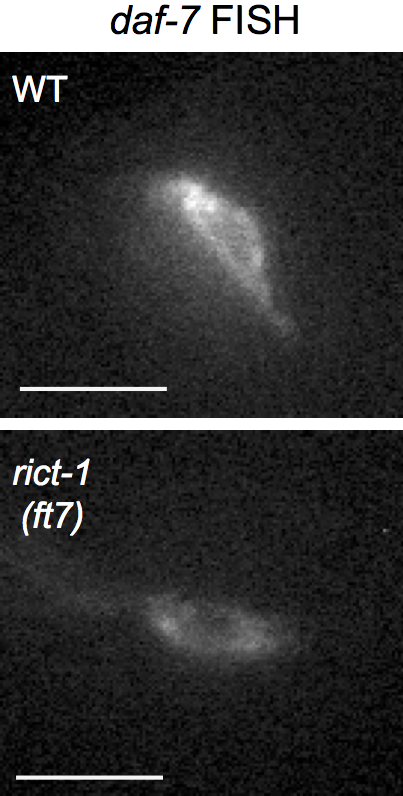
\includegraphics[width=5.6in]{/Users/mikeod/git/projects/dauergut/figures/S1A_daf7FISH}

\subsection{S1B}\label{s1b}

\begin{Shaded}
\begin{Highlighting}[]
\NormalTok{strains<-}\KeywordTok{c}\NormalTok{(}\StringTok{"N2"}\NormalTok{,}\StringTok{"mg360"}\NormalTok{)}
\NormalTok{conc.adjust <-}\DecValTok{15}
\NormalTok{dates<-}\KeywordTok{c}\NormalTok{(}\StringTok{"8_10_16"}\NormalTok{)}
\NormalTok{d7GFP<-}\KeywordTok{read.csv}\NormalTok{(}\KeywordTok{file.path}\NormalTok{(pathname,}\StringTok{"extdata"}\NormalTok{,}\StringTok{"2A_3A_daf7GFP.csv"}\NormalTok{)) }\OperatorTok\StringTok{ }\KeywordTok{filter}\NormalTok{(mean}\OperatorTok{!=}\DecValTok{4095} \OperatorTok{&}\StringTok{ }\NormalTok{genotype }\OperatorTok\StringTok{ }\NormalTok{strains }\OperatorTok{&}\StringTok{ }\NormalTok{date }\OperatorTok\StringTok{ }\NormalTok{dates }\OperatorTok{&}\StringTok{ }\NormalTok{temp }\OperatorTok{==}\StringTok{ "25"} \OperatorTok{&}\StringTok{ }\NormalTok{food }\OperatorTok{==}\StringTok{ "OP50"}\NormalTok{) }\OperatorTok\StringTok{ }\KeywordTok{mutate}\NormalTok{(}\DataTypeTok{genotype =} \KeywordTok{factor}\NormalTok{(genotype, }\DataTypeTok{levels=}\NormalTok{strains), }\DataTypeTok{ID =} \KeywordTok{as.character}\NormalTok{(ID)) }\OperatorTok
\StringTok{  }\KeywordTok{separate}\NormalTok{(ID, }\KeywordTok{c}\NormalTok{(}\StringTok{"ID.A"}\NormalTok{, }\StringTok{"ID.B"}\NormalTok{), }\DataTypeTok{sep =} \StringTok{":"}\NormalTok{, }\DataTypeTok{extra =} \StringTok{"drop"}\NormalTok{) }\OperatorTok\StringTok{ }
\StringTok{  }\KeywordTok{mutate}\NormalTok{(}\DataTypeTok{genoID =} \KeywordTok{paste}\NormalTok{(date, genotype, ID.A, }\DataTypeTok{sep =} \StringTok{":"}\NormalTok{), }\DataTypeTok{cell.norm =}\NormalTok{ mean, }\DataTypeTok{adj.pheromone =}\NormalTok{ pheromone }\OperatorTok{+}\StringTok{ }\NormalTok{conc.adjust, }
         \DataTypeTok{inv.pher =} \DecValTok{1}\OperatorTok{/}\NormalTok{adj.pheromone) }\CommentTok{#genoID is animal, 2 cells per animal measured.}

\NormalTok{df <-}\StringTok{ }\NormalTok{d7GFP }\OperatorTok\StringTok{ }\KeywordTok{group_by}\NormalTok{(date, genotype, genoID, adj.pheromone) }\OperatorTok\StringTok{ }\KeywordTok{summarise}\NormalTok{(}\DataTypeTok{cell.norm =} \KeywordTok{mean}\NormalTok{(cell.norm))}

\NormalTok{log.tran<-lsmeans}\OperatorTok{::}\KeywordTok{make.tran}\NormalTok{(}\DataTypeTok{type=}\StringTok{"genlog"}\NormalTok{, }\DataTypeTok{param =} \KeywordTok{c}\NormalTok{(}\DecValTok{0}\NormalTok{,}\DecValTok{10}\NormalTok{))}

\CommentTok{#convert to proportion:}
\NormalTok{lm <-}\StringTok{ }\KeywordTok{lm}\NormalTok{(cell.norm }\OperatorTok{~}\StringTok{ }\NormalTok{genotype }\OperatorTok{+}\StringTok{ }\NormalTok{adj.pheromone,  }\DataTypeTok{data =}\NormalTok{ df)}
\NormalTok{lm1<-}\StringTok{ }\KeywordTok{lm}\NormalTok{(cell.norm }\OperatorTok{~}\StringTok{ }\NormalTok{genotype }\OperatorTok{+}\StringTok{ }\KeywordTok{poly}\NormalTok{(adj.pheromone,}\DecValTok{2}\NormalTok{),  }\DataTypeTok{data =}\NormalTok{ df)}
\NormalTok{lm2 <-}\StringTok{ }\KeywordTok{lm}\NormalTok{(cell.norm }\OperatorTok{~}\StringTok{ }\NormalTok{genotype }\OperatorTok{*}\StringTok{ }\KeywordTok{poly}\NormalTok{(adj.pheromone, }\DecValTok{2}\NormalTok{), }\DataTypeTok{data =}\NormalTok{ df)}

\CommentTok{# stanlmer <- with(log.tran, rstanarm::stan_lmer(linkfun(cell.norm) ~ genotype + (1|date) + (1:genotype:date),}
\CommentTok{#                                                data = df,}
\CommentTok{#                                                chains = 3,}
\CommentTok{#                                                cores =4,}
\CommentTok{#                                                seed = 2000,}
\CommentTok{#                                                iter=6000,}
\CommentTok{#                                                control = list(adapt_delta=0.99)))}


\NormalTok{newdata =}\StringTok{ }\KeywordTok{data.frame}\NormalTok{(}\DataTypeTok{genotype =} \KeywordTok{rep}\NormalTok{(strains, }\DataTypeTok{each =} \DecValTok{241}\NormalTok{), }\DataTypeTok{adj.pheromone =} \KeywordTok{rep}\NormalTok{(}\KeywordTok{seq}\NormalTok{(}\DecValTok{10}\NormalTok{,}\DecValTok{2410}\NormalTok{, }\DataTypeTok{by =} \DecValTok{10}\NormalTok{),}\DecValTok{2}\NormalTok{),}\DataTypeTok{genoID =} \KeywordTok{rep}\NormalTok{(}\DecValTok{0}\NormalTok{, }\DecValTok{482}\NormalTok{))}

\NormalTok{### for non-interaction }\AlertTok{###} 
\CommentTok{#glm.simple <- glm(data = rictC3, cbind(dauer, non) ~ concentration.uM. + genotype, family = binomial)}
\NormalTok{predictions <-}\StringTok{ }\KeywordTok{predict}\NormalTok{(lm, }\DataTypeTok{newdata =}\NormalTok{ newdata, }\DataTypeTok{type =} \StringTok{"response"}\NormalTok{, }\DataTypeTok{se.fit =} \OtherTok{TRUE}\NormalTok{)}
\NormalTok{predictions.}\DecValTok{2}\NormalTok{ <-}\StringTok{ }\KeywordTok{predict}\NormalTok{(lm2, }\DataTypeTok{newdata =}\NormalTok{ newdata, }\DataTypeTok{type =} \StringTok{"response"}\NormalTok{, }\DataTypeTok{se.fit =} \OtherTok{TRUE}\NormalTok{)}
\NormalTok{newdata1 <-}\StringTok{ }\KeywordTok{cbind}\NormalTok{(newdata, predictions.}\DecValTok{2}\NormalTok{)}
\NormalTok{newdata1 }\OperatorTok\StringTok{ }\KeywordTok{mutate}\NormalTok{(}\DataTypeTok{lower =}\NormalTok{ (fit }\OperatorTok{-}\StringTok{ }\NormalTok{se.fit), }\DataTypeTok{upper =}\NormalTok{ (fit }\OperatorTok{+}\StringTok{ }\NormalTok{se.fit), }\DataTypeTok{AU =}\NormalTok{ fit, }\DataTypeTok{genotype =} \KeywordTok{factor}\NormalTok{(genotype, }\DataTypeTok{levels =}\NormalTok{ strains))}


\NormalTok{(p<-df }\OperatorTok\StringTok{ }\NormalTok{ungroup }\OperatorTok\StringTok{ }\KeywordTok{ggplot}\NormalTok{(}\KeywordTok{aes}\NormalTok{(}\DataTypeTok{x=}\NormalTok{ adj.pheromone)) }\OperatorTok{+}
\StringTok{    }\KeywordTok{geom_ribbon}\NormalTok{(}\DataTypeTok{data =}\NormalTok{ newdata1,}\KeywordTok{aes}\NormalTok{(}\DataTypeTok{ymin=}\NormalTok{lower, }\DataTypeTok{ymax=}\NormalTok{upper, }\DataTypeTok{fill=}\NormalTok{genotype), }\DataTypeTok{alpha=}\FloatTok{0.3}\NormalTok{) }\OperatorTok{+}
\StringTok{    }\KeywordTok{geom_line}\NormalTok{(}\DataTypeTok{data =}\NormalTok{ newdata1,}\KeywordTok{aes}\NormalTok{(}\DataTypeTok{x =}\NormalTok{  adj.pheromone, }\DataTypeTok{y =}\NormalTok{ AU, }\DataTypeTok{colour =}\NormalTok{ genotype)) }\OperatorTok{+}
\StringTok{    }\KeywordTok{add.median}\NormalTok{(}\DataTypeTok{width =} \DecValTok{150}\NormalTok{) }\OperatorTok{+}
\StringTok{    }\KeywordTok{add.quartiles}\NormalTok{(}\DataTypeTok{width =} \DecValTok{60}\NormalTok{) }\OperatorTok{+}
\StringTok{    }\KeywordTok{geom_quasirandom}\NormalTok{(}\KeywordTok{aes}\NormalTok{(}\DataTypeTok{y=}\NormalTok{cell.norm),}\DataTypeTok{colour =} \StringTok{"#339900"}\NormalTok{, }\DataTypeTok{cex=}\DecValTok{1}\NormalTok{,}
                           \DataTypeTok{width =} \DecValTok{40}\NormalTok{,}\DataTypeTok{size=}\FloatTok{0.3}\NormalTok{,}
                           \DataTypeTok{method =} \StringTok{'smiley'}\NormalTok{) }\OperatorTok{+}
\StringTok{    }\KeywordTok{labs}\NormalTok{(}\DataTypeTok{y =} \StringTok{"GFP intensity (AU)"}\NormalTok{,}
         \DataTypeTok{x =} \StringTok{"ascr#5 concentration (nM)"}\NormalTok{) }\OperatorTok{+}
\StringTok{    }\KeywordTok{facet_grid}\NormalTok{(.}\OperatorTok{~}\NormalTok{genotype) }\OperatorTok{+}
\StringTok{    }\KeywordTok{scale_fill_manual}\NormalTok{(}\DataTypeTok{values =} \KeywordTok{c}\NormalTok{(}\StringTok{"grey"}\NormalTok{, }\StringTok{"lightblue"}\NormalTok{)) }\OperatorTok{+}
\StringTok{    }\KeywordTok{scale_colour_manual}\NormalTok{(}\DataTypeTok{values =} \KeywordTok{c}\NormalTok{(}\StringTok{"grey"}\NormalTok{, }\StringTok{"lightblue"}\NormalTok{)) }\OperatorTok{+}
\StringTok{  }\KeywordTok{geom_text}\NormalTok{(}\KeywordTok{aes}\NormalTok{(}\DataTypeTok{y =} \FloatTok{1.075}\NormalTok{, }\DataTypeTok{x=}\NormalTok{ adj.pheromone), }\DataTypeTok{label =} \StringTok{""}\NormalTok{) }\OperatorTok{+}
\StringTok{  }\KeywordTok{theme_classic}\NormalTok{() }\OperatorTok{+}
\StringTok{  }\KeywordTok{theme}\NormalTok{(}
        \DataTypeTok{axis.text.x=}\KeywordTok{element_text}\NormalTok{(}\DataTypeTok{angle=}\DecValTok{45}\NormalTok{, }\DataTypeTok{hjust=}\DecValTok{1}\NormalTok{, }\DataTypeTok{size=}\DecValTok{12}\NormalTok{),}
        \DataTypeTok{axis.text.y =} \KeywordTok{element_text}\NormalTok{(}\DataTypeTok{size=}\DecValTok{16}\NormalTok{),}
        \DataTypeTok{axis.title.y =} \KeywordTok{element_text}\NormalTok{(}\DataTypeTok{size =}\DecValTok{20}\NormalTok{),}
        \DataTypeTok{axis.title.x =} \KeywordTok{element_text}\NormalTok{(}\DataTypeTok{size=}\DecValTok{16}\NormalTok{),}
        \DataTypeTok{strip.text.x =} \KeywordTok{element_blank}\NormalTok{(),}
        \DataTypeTok{panel.spacing =} \KeywordTok{unit}\NormalTok{(}\DecValTok{2}\NormalTok{,}\StringTok{"lines"}\NormalTok{)) }\OperatorTok{+}
\StringTok{    }\KeywordTok{stat_summary}\NormalTok{(}\KeywordTok{aes}\NormalTok{(}\DataTypeTok{x=}\NormalTok{ adj.pheromone }\OperatorTok{+}\StringTok{ }\FloatTok{0.3}\NormalTok{, }\DataTypeTok{y=}\OperatorTok{-}\NormalTok{.}\DecValTok{025}\NormalTok{),}
                      \DataTypeTok{fun.data =}\NormalTok{ fun_length, }\DataTypeTok{geom =} \StringTok{"text"}\NormalTok{, }\DataTypeTok{size =} \DecValTok{4}\NormalTok{))}
\end{Highlighting}
\end{Shaded}

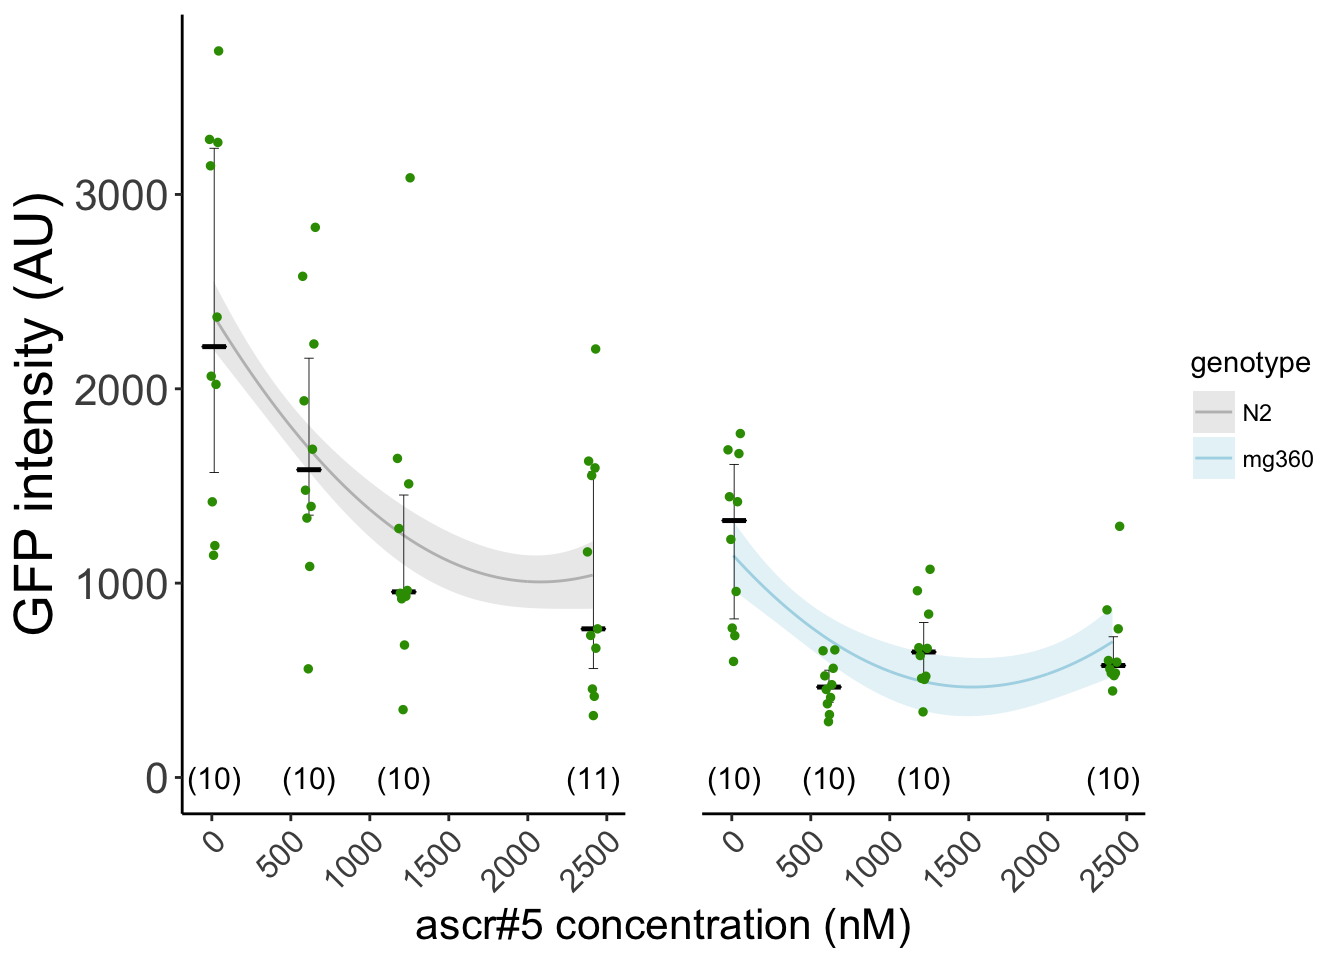
\includegraphics{Figure_2_files/figure-latex/daf7 pheromone response-1.pdf}

\textbf{Figure S1B} \emph{rict-1} mutants show enhanced response to
pheromone ascr\#5. \emph{daf-7::}GFP expression in wild-type (black) and
rict-1(mg360) (blue) animals at 25°C in the presence of the indicated
concentrations of ascr\#5 and live OP50. Each dot indicates the average
ASI GFP intensity in each each animal (2 neurons per animal). Horizontal
bar indicates median, error bars indicate quartiles. The number of
animals are indicated in parentheses. Lines indicate predictions from
quadratic fit.

\begin{Shaded}
\begin{Highlighting}[]
\KeywordTok{library}\NormalTok{(sjPlot)}
\KeywordTok{sjt.lm}\NormalTok{(lm2, }\DataTypeTok{depvar.labels =} \StringTok{"proportion of dauers"}\NormalTok{, }\DataTypeTok{show.se =} \OtherTok{TRUE}\NormalTok{, }\DataTypeTok{show.fstat =} \OtherTok{TRUE}\NormalTok{)}
\end{Highlighting}
\end{Shaded}

~

~

proportion of dauers

~

~

B

CI

std. Error

p

(Intercept)

~

1581.53

1400.91~--~1762.16

90.67

\textless{}.001

genotypemg360

~

-821.95

-1078.99~--~-564.91

129.03

\textless{}.001

poly(adj.pheromone, 2)1

~

-4209.77

-5823.52~--~-2596.03

810.07

\textless{}.001

poly(adj.pheromone, 2)2

~

1838.23

208.73~--~3467.72

817.98

.028

genotypemg360:poly(adj.pheromone, 2)1

~

2975.46

661.29~--~5289.64

1161.67

.012

genotypemg360:poly(adj.pheromone, 2)2

~

-141.83

-2454.91~--~2171.25

1161.12

.903

Observations

~

81

R2 / adj. R2

~

.510 / .478

F-statistics

~

15.629***

\subsection{S1C}\label{s1c}

\begin{Shaded}
\begin{Highlighting}[]
\NormalTok{strains <-}\StringTok{ }\KeywordTok{c}\NormalTok{(}\StringTok{"N2"}\NormalTok{, }\StringTok{"rict-1(ft7)"}\NormalTok{)}
\NormalTok{foods <-}\StringTok{ "OP50"}
\NormalTok{rictC3 <-}\StringTok{ }\KeywordTok{read.csv}\NormalTok{(}\KeywordTok{file.path}\NormalTok{(pathname, }\StringTok{'extdata'}\NormalTok{,}\StringTok{'S1C_rict1Pheromone.csv'}\NormalTok{)) }\OperatorTok\StringTok{ }\KeywordTok{format_dauer}\NormalTok{(}\DataTypeTok{p.dauer =} \StringTok{"exclude"}\NormalTok{) }\OperatorTok\StringTok{ }\KeywordTok{mutate}\NormalTok{(}\DataTypeTok{plateID =} \KeywordTok{interaction}\NormalTok{(plateID,concentration.uM.)) }

\CommentTok{# for glm fit}
\NormalTok{glm <-}\StringTok{ }\KeywordTok{glm}\NormalTok{(}\DataTypeTok{data =}\NormalTok{ rictC3, }\KeywordTok{cbind}\NormalTok{(dauer, non) }\OperatorTok{~}\StringTok{ }\NormalTok{concentration.uM. }\OperatorTok{+}\StringTok{ }\NormalTok{genotype }\OperatorTok{+}\StringTok{ }\NormalTok{concentration.uM. }\OperatorTok{*}\StringTok{ }\NormalTok{genotype, }\DataTypeTok{family =}\NormalTok{ binomial)}

\NormalTok{newdata =}\StringTok{ }\KeywordTok{data.frame}\NormalTok{(}\DataTypeTok{genotype =} \KeywordTok{rep}\NormalTok{(strains, }\DataTypeTok{each =} \DecValTok{241}\NormalTok{), }\DataTypeTok{concentration.uM. =} \KeywordTok{rep}\NormalTok{(}\KeywordTok{seq}\NormalTok{(}\DecValTok{0}\NormalTok{,}\FloatTok{2.4}\NormalTok{, }\DataTypeTok{by =} \FloatTok{0.01}\NormalTok{),}\DecValTok{2}\NormalTok{),}\DataTypeTok{plateID =} \KeywordTok{rep}\NormalTok{(}\DecValTok{0}\NormalTok{, }\DecValTok{482}\NormalTok{), }\DataTypeTok{n =} \KeywordTok{rep}\NormalTok{(}\DecValTok{60}\NormalTok{, }\DecValTok{482}\NormalTok{))}

\NormalTok{### for non-interaction }\AlertTok{###} 
\NormalTok{glm.simple <-}\StringTok{ }\KeywordTok{glm}\NormalTok{(}\DataTypeTok{data =}\NormalTok{ rictC3, }\KeywordTok{cbind}\NormalTok{(dauer, non) }\OperatorTok{~}\StringTok{ }\NormalTok{concentration.uM. }\OperatorTok{+}\StringTok{ }\NormalTok{genotype, }\DataTypeTok{family =}\NormalTok{ binomial)}
\NormalTok{predictions <-}\StringTok{ }\KeywordTok{predict}\NormalTok{(glm, }\DataTypeTok{newdata =}\NormalTok{ newdata, }\DataTypeTok{type =} \StringTok{"response"}\NormalTok{, }\DataTypeTok{se.fit =} \OtherTok{TRUE}\NormalTok{)}
\NormalTok{newdata1 <-}\StringTok{ }\KeywordTok{cbind}\NormalTok{(newdata, predictions)}
\NormalTok{newdata1 }\OperatorTok\StringTok{ }\KeywordTok{mutate}\NormalTok{(}\DataTypeTok{lower =}\NormalTok{ (fit }\OperatorTok{-}\StringTok{ }\NormalTok{se.fit), }\DataTypeTok{upper =}\NormalTok{ (fit }\OperatorTok{+}\StringTok{ }\NormalTok{se.fit), }\DataTypeTok{pct =}\NormalTok{ fit)}


\NormalTok{(p<-rictC3 }\OperatorTok\StringTok{ }\KeywordTok{ggplot}\NormalTok{(}\KeywordTok{aes}\NormalTok{(}\DataTypeTok{x=}\NormalTok{concentration.uM.,}\DataTypeTok{y =}\NormalTok{ pct)) }\OperatorTok{+}
\StringTok{  }\KeywordTok{geom_ribbon}\NormalTok{(}\DataTypeTok{data =}\NormalTok{ newdata1,}\KeywordTok{aes}\NormalTok{(}\DataTypeTok{ymin=}\NormalTok{lower, }\DataTypeTok{ymax=}\NormalTok{upper,}\DataTypeTok{fill=}\NormalTok{genotype), }\DataTypeTok{alpha=}\FloatTok{0.3}\NormalTok{) }\OperatorTok{+}
\StringTok{  }\KeywordTok{geom_line}\NormalTok{(}\DataTypeTok{data =}\NormalTok{ newdata1,}\KeywordTok{aes}\NormalTok{(}\DataTypeTok{x =}\NormalTok{ concentration.uM., }\DataTypeTok{y =}\NormalTok{ pct, }\DataTypeTok{colour =}\NormalTok{ genotype)) }\OperatorTok{+}
\StringTok{  }\KeywordTok{geom_point}\NormalTok{(}\KeywordTok{aes}\NormalTok{(}\DataTypeTok{y=}\NormalTok{pct), }\DataTypeTok{size =} \FloatTok{0.6}\NormalTok{, }\DataTypeTok{alpha =} \FloatTok{0.75}\NormalTok{) }\OperatorTok{+}
\StringTok{  }\KeywordTok{add.median.dauer}\NormalTok{() }\OperatorTok{+}
\StringTok{  }\KeywordTok{labs}\NormalTok{(}\DataTypeTok{y =} \StringTok{"proportion dauer"}\NormalTok{, }
       \DataTypeTok{x =} \StringTok{"ascr#5 concentration (uM)"}\NormalTok{) }\OperatorTok{+}
\StringTok{  }\KeywordTok{facet_grid}\NormalTok{(.}\OperatorTok{~}\NormalTok{genotype) }\OperatorTok{+}
\StringTok{  }\KeywordTok{scale_fill_manual}\NormalTok{(}\DataTypeTok{values =} \KeywordTok{c}\NormalTok{(}\StringTok{"grey"}\NormalTok{, }\StringTok{"lightblue"}\NormalTok{)) }\OperatorTok{+}
\StringTok{  }\KeywordTok{scale_colour_manual}\NormalTok{(}\DataTypeTok{values =} \KeywordTok{c}\NormalTok{(}\StringTok{"grey"}\NormalTok{, }\StringTok{"lightblue"}\NormalTok{)) }\OperatorTok{+}
\StringTok{  }\KeywordTok{geom_text}\NormalTok{(}\KeywordTok{aes}\NormalTok{(}\DataTypeTok{y =} \FloatTok{1.075}\NormalTok{, }\DataTypeTok{x=}\NormalTok{concentration.uM.), }\DataTypeTok{label =} \StringTok{""}\NormalTok{) }\OperatorTok{+}
\StringTok{    }\KeywordTok{coord_cartesian}\NormalTok{(}\DataTypeTok{ylim =} \KeywordTok{c}\NormalTok{(}\OperatorTok{-}\NormalTok{.}\DecValTok{005}\NormalTok{,}\FloatTok{1.075}\NormalTok{)) }\OperatorTok{+}
\StringTok{      }\KeywordTok{scale_y_continuous}\NormalTok{(}\DataTypeTok{breaks=}\KeywordTok{c}\NormalTok{(}\DecValTok{0}\NormalTok{,}\FloatTok{0.25}\NormalTok{,}\FloatTok{0.5}\NormalTok{,}\FloatTok{0.75}\NormalTok{,}\DecValTok{1}\NormalTok{)) }\OperatorTok{+}
\StringTok{  }\KeywordTok{theme_classic}\NormalTok{() }\OperatorTok{+}
\StringTok{  }\KeywordTok{theme}\NormalTok{(}
        \DataTypeTok{axis.text.x =} \KeywordTok{element_text}\NormalTok{(}\DataTypeTok{size=}\DecValTok{16}\NormalTok{),}
        \DataTypeTok{axis.text.y =} \KeywordTok{element_text}\NormalTok{(}\DataTypeTok{size=}\DecValTok{16}\NormalTok{),}
        \DataTypeTok{axis.title.y =} \KeywordTok{element_text}\NormalTok{(}\DataTypeTok{size =}\DecValTok{20}\NormalTok{),}
        \DataTypeTok{axis.title.x =} \KeywordTok{element_text}\NormalTok{(}\DataTypeTok{size=}\DecValTok{16}\NormalTok{),}
        \DataTypeTok{strip.text.x =} \KeywordTok{element_blank}\NormalTok{(),}
        \DataTypeTok{panel.spacing =} \KeywordTok{unit}\NormalTok{(}\DecValTok{2}\NormalTok{,}\StringTok{"lines"}\NormalTok{)) }\OperatorTok{+}
\StringTok{    }\KeywordTok{stat_summary}\NormalTok{(}\KeywordTok{aes}\NormalTok{(}\DataTypeTok{x=}\NormalTok{concentration.uM. }\OperatorTok{+}\StringTok{ }\FloatTok{0.3}\NormalTok{, }\DataTypeTok{y=}\OperatorTok{-}\NormalTok{.}\DecValTok{025}\NormalTok{),}
                      \DataTypeTok{fun.data =}\NormalTok{ fun_length, }\DataTypeTok{geom =} \StringTok{"text"}\NormalTok{, }\DataTypeTok{size =} \DecValTok{4}\NormalTok{)}
\NormalTok{)}
\end{Highlighting}
\end{Shaded}

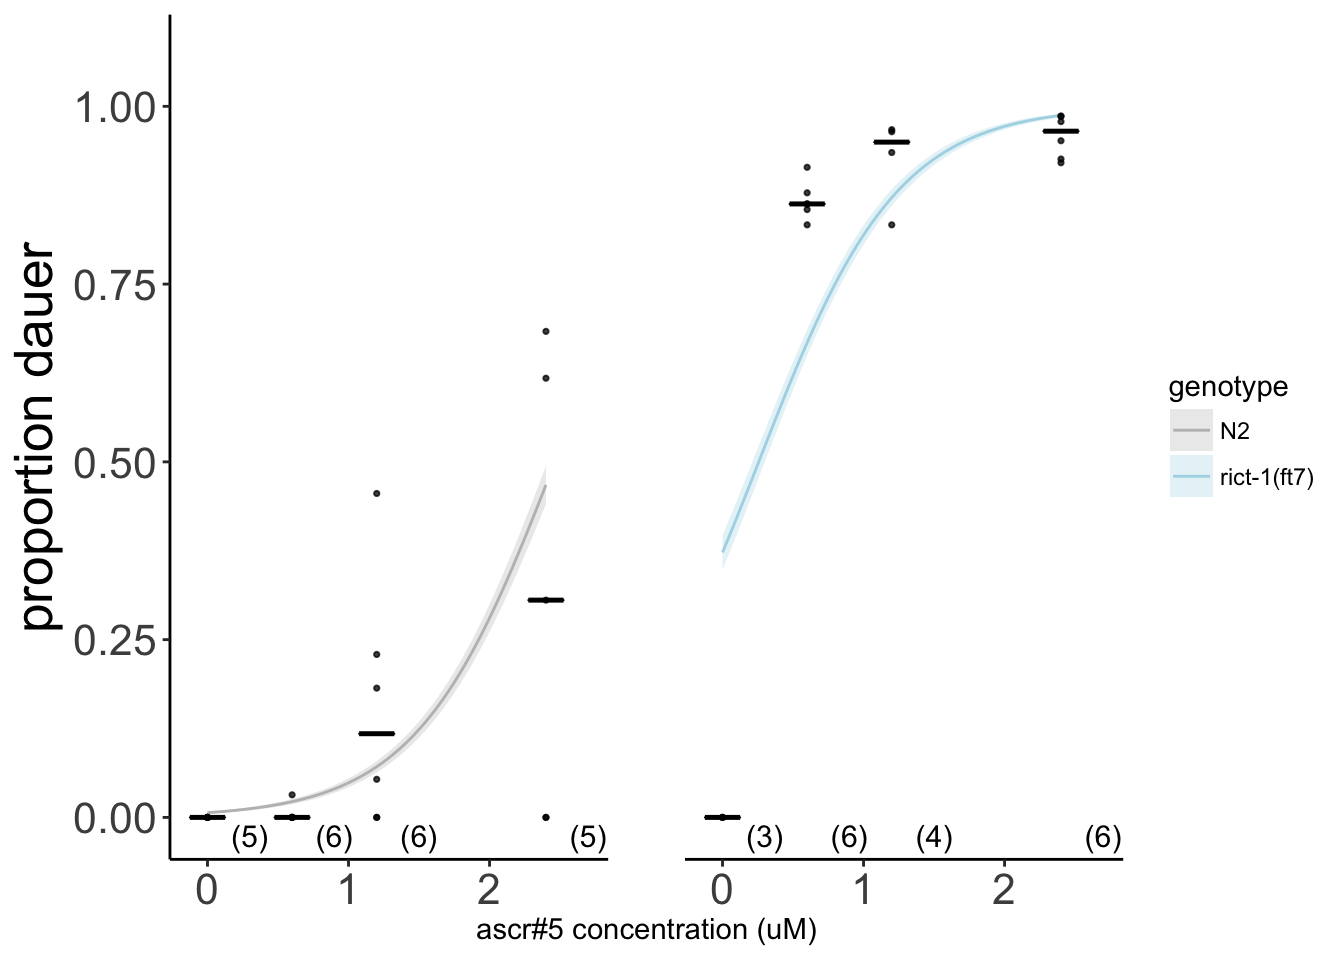
\includegraphics{Figure_2_files/figure-latex/rict-1 pheromone response-1.pdf}

\textbf{Figure S1C} \emph{rict-1} mutants show enhanced response to
pheromone ascr\#5. Dauers formed by wild-type (black) and rict-1(ft7)
(blue) animals at 25°C in the presence of the indicated concentrations
of ascr\#5. Each dot indicates the proportion of dauers formed in a
single assay. Horizontal bar indicates median. Numbers in parentheses
below indicate the number of independent experiments with at least 27
animals each. Lines indicate predictions from GLM fit, corresponding to
an odds ratio of \texttt{as.numeric(round(exp(coef(glm)){[}3{]},1))} for
rict-1 across this range of ascr\#5 concentrations.

\begin{Shaded}
\begin{Highlighting}[]
\KeywordTok{library}\NormalTok{(sjPlot)}
\KeywordTok{sjt.glm}\NormalTok{(glm, }\DataTypeTok{depvar.labels =} \StringTok{"proportion of dauers"}\NormalTok{, }\DataTypeTok{show.se =} \OtherTok{TRUE}\NormalTok{, }\DataTypeTok{show.chi2 =} \OtherTok{TRUE}\NormalTok{)}
\end{Highlighting}
\end{Shaded}

~

~

proportion of dauers

~

~

Odds Ratio

CI

std. Error

p

(Intercept)

~

0.02

0.01~--~0.02

0.00

\textless{}.001

concentration.uM.

~

4.79

3.83~--~6.05

0.56

\textless{}.001

genotyperict-1(ft7)

~

21.28

12.69~--~36.47

5.72

\textless{}.001

concentration.uM.:genotyperict-1(ft7)

~

4.41

2.73~--~7.35

1.11

\textless{}.001

Observations

~

41

Χ2deviance

~

p=.000

\subsection{S1D}\label{s1d}

\begin{Shaded}
\begin{Highlighting}[]
\NormalTok{foods <-}\StringTok{ "OP50"}
\NormalTok{strains<-}\KeywordTok{c}\NormalTok{(}\StringTok{"N2"}\NormalTok{,}\StringTok{"rict-1(ft7)"}\NormalTok{,}\StringTok{"rict-1(ft7); ex[ASI::daf7]"}\NormalTok{,}\StringTok{"rict-1(ft7); ex[ASI::daf28]"}\NormalTok{,}\StringTok{"rict-1(ft7); ex[ASJ::daf28]"}\NormalTok{)}
\NormalTok{daf7supp<-}\KeywordTok{read.csv}\NormalTok{(}\KeywordTok{file.path}\NormalTok{(pathname, }\StringTok{"extdata"}\NormalTok{,}\StringTok{"S1D_daf7_daf28_suppression.csv"}\NormalTok{)) }\OperatorTok\StringTok{ }\KeywordTok{format_dauer}\NormalTok{(}\DataTypeTok{p.dauer =} \StringTok{"non"}\NormalTok{)}

\CommentTok{# daf7supp$genotype<- factor(daf7supp$genotype, levels = strains)}
\CommentTok{# daf7supp$pct<-as.numeric(paste(daf7supp$dauer/(daf7supp$dauer+daf7supp$pd + daf7supp$non))) #omitted arrest}
\CommentTok{# daf7supp$non.dauer<-as.numeric(paste(daf7supp$pd+daf7supp$non))}

\NormalTok{lm <-}\StringTok{ }\NormalTok{daf7supp }\OperatorTok\StringTok{ }\KeywordTok{dauer_ANOVA}\NormalTok{()}
\CommentTok{#stan}
\NormalTok{stan.glmm <-}\StringTok{ }\NormalTok{daf7supp }\OperatorTok\StringTok{ }\NormalTok{dauergut}\OperatorTok{::}\KeywordTok{run_dauer_stan}\NormalTok{()}
\end{Highlighting}
\end{Shaded}

\begin{Shaded}
\begin{Highlighting}[]
\NormalTok{foods <-}\StringTok{ "OP50"}
\NormalTok{contrasts<-dauergut}\OperatorTok{::}\KeywordTok{tukey_contrasts}\NormalTok{(lm, }\StringTok{"genotype"}\NormalTok{)}
\NormalTok{mixed<-stan.glmm }\OperatorTok\StringTok{ }\NormalTok{dauergut}\OperatorTok{::}\KeywordTok{getStan_CIs}\NormalTok{(}\DataTypeTok{type =} \StringTok{"dauer"}\NormalTok{)}
\NormalTok{plot.contrasts<-}\KeywordTok{c}\NormalTok{(}\StringTok{""}\NormalTok{,contrasts}\OperatorTok{$}\NormalTok{prange[}\DecValTok{1}\NormalTok{],}\StringTok{""}\NormalTok{,}\StringTok{""}\NormalTok{,}\StringTok{""}\NormalTok{)}
\NormalTok{plot.contrasts.}\DecValTok{2}\NormalTok{<-}\KeywordTok{c}\NormalTok{(}\StringTok{""}\NormalTok{, }\StringTok{""}\NormalTok{, contrasts}\OperatorTok{$}\NormalTok{prange[}\DecValTok{5}\OperatorTok{:}\DecValTok{7}\NormalTok{]) }\CommentTok{#for rescue vs rict-1}

\NormalTok{labels <-}\StringTok{ }\KeywordTok{c}\NormalTok{(}\StringTok{"WT"}\NormalTok{,}\StringTok{"rict-1(ft7)"}\NormalTok{,}\StringTok{"rict-1(ft7); +ASIp::daf-7"}\NormalTok{,}\StringTok{"rict-1(ft7); +ASIp::daf-28"}\NormalTok{,}\StringTok{"rict-1(ft7); +ASJp::daf-28"}\NormalTok{) }\OperatorTok\StringTok{ }\NormalTok{stringr}\OperatorTok{::}\KeywordTok{str_wrap}\NormalTok{(}\DataTypeTok{width =} \DecValTok{10}\NormalTok{)}


\NormalTok{p<-dauergut}\OperatorTok{::}\KeywordTok{plot_CIs}\NormalTok{(daf7supp, }\DataTypeTok{title=}\StringTok{'daf-7 expression in ASI suppresses rict-1 dauer phenotype'}\NormalTok{, plot.contrasts, plot.contrasts.}\DecValTok{2}\NormalTok{, }\DataTypeTok{ypos =} \FloatTok{1.075}\NormalTok{, }\DataTypeTok{offset =} \DecValTok{0}\NormalTok{, }\DataTypeTok{type =} \StringTok{"dauer"}\NormalTok{, }\DataTypeTok{labels =}\NormalTok{ labels)}
\end{Highlighting}
\end{Shaded}

\begin{Shaded}
\begin{Highlighting}[]
\NormalTok{p}
\end{Highlighting}
\end{Shaded}

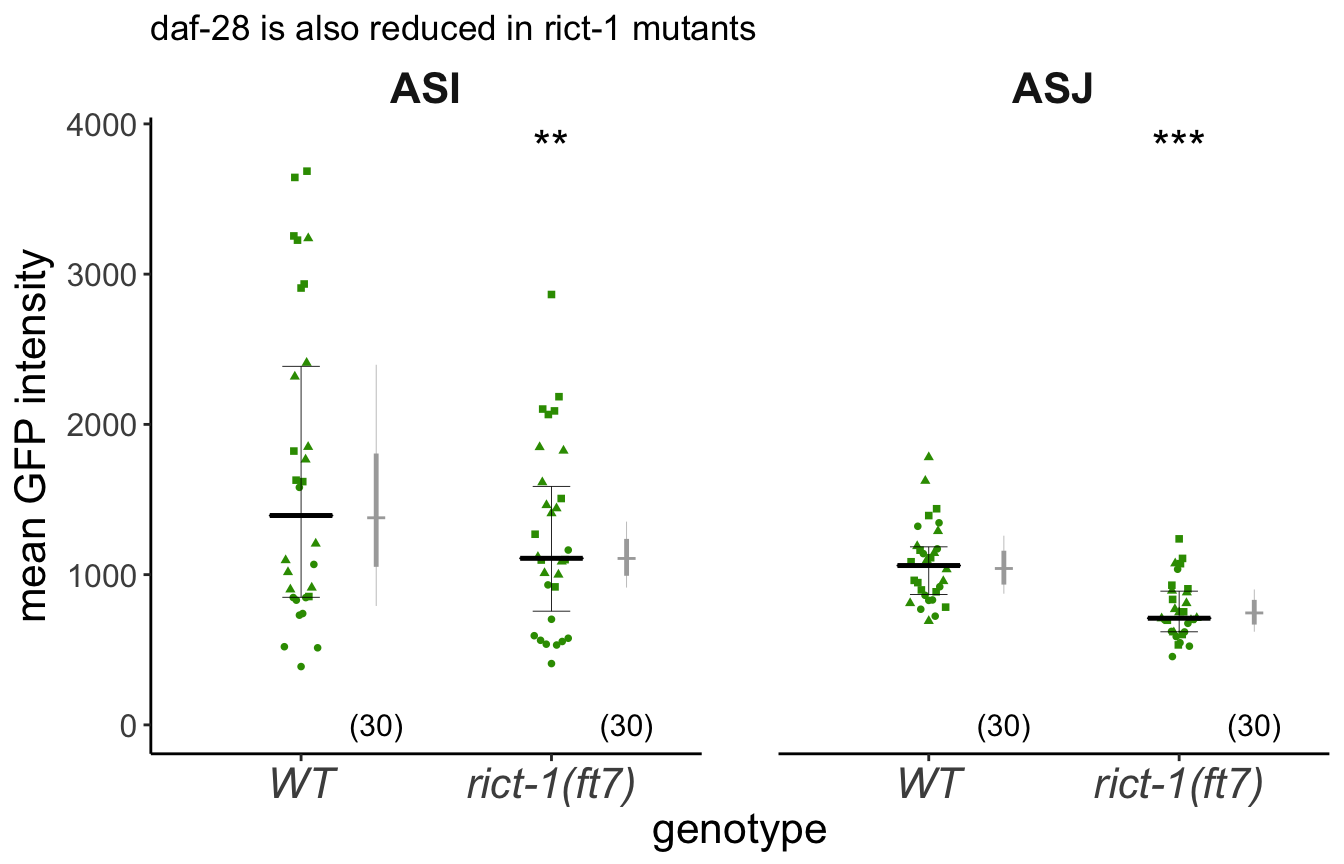
\includegraphics{Figure_2_files/figure-latex/unnamed-chunk-5-1.pdf}

 \textbf{Figure 2C} Expression of \emph{daf-7} in ASI or \emph{daf-28}
in ASI or ASJ suppressed aberrent dauer formation in \emph{rict-1}
mutants. Dauers formed by animals of the indicated genotypes at 27°C.
Each black dot indicates the average number of dauers formed in a single
assay. Horizontal black bar indicates median. Light gray thin and thick
vertical bars at right indicate Bayesian 95\% and 75\% credible
intervals, respectively. Numbers in parentheses below indicate the
number of independent experiments with at least 36 and 9 animals each
scored for non-transgenic and transgenic animals, respectively.
Promoters driving expression in ASI and ASJ were \emph{srg-47p} and
\emph{trx-1p}, respectively. One transgenic line was tested for each
condition. {\texttt{***}} - different from wild-type at
P\textless{}0.001; {\texttt{**}} and {\texttt{***}} - different from
\emph{rict-1(ft7)} at P\textless{}0.01 and P\textless{}0.001,
respectively (ANOVA with Tukey-type multivariate-t post-hoc adjustment).
P-values of differences in means relative to wild-type and corresponding
mutant animals are indicated in black and red, respectively.

\begin{Shaded}
\begin{Highlighting}[]
\KeywordTok{library}\NormalTok{(sjPlot)}
\KeywordTok{sjt.lm}\NormalTok{(lm, }\DataTypeTok{depvar.labels =} \StringTok{"proportion of dauers"}\NormalTok{, }\DataTypeTok{show.se =} \OtherTok{TRUE}\NormalTok{, }\DataTypeTok{show.fstat =} \OtherTok{TRUE}\NormalTok{)}
\end{Highlighting}
\end{Shaded}

~

~

proportion of dauers

~

~

B

CI

std. Error

p

(Intercept)

~

0.07

-0.13~--~0.26

0.09

.493

genotype

rict-1(ft7)

~

0.89

0.61~--~1.17

0.13

\textless{}.001

rict-1(ft7); ex{[}ASI::daf7{]}

~

0.23

-0.04~--~0.51

0.13

.094

rict-1(ft7); ex{[}ASI::daf28{]}

~

-0.01

-0.32~--~0.31

0.15

.971

rict-1(ft7); ex{[}ASJ::daf28{]}

~

0.37

0.09~--~0.65

0.13

.012

Observations

~

28

R2 / adj. R2

~

.709 / .658

F-statistics

~

14.007***

\begin{Shaded}
\begin{Highlighting}[]
\NormalTok{knitr}\OperatorTok{::}\KeywordTok{kable}\NormalTok{(contrasts, }\DataTypeTok{caption=}\StringTok{"Pairwise comparisons from ANOVA (Tukey)"}\NormalTok{)}
\end{Highlighting}
\end{Shaded}

\begin{longtable}[]{@{}lrrrrrl@{}}
\caption{Pairwise comparisons from ANOVA (Tukey)}\tabularnewline
\toprule
contrast & estimate & SE & df & t.ratio & p.value &
prange\tabularnewline
\midrule
\endfirsthead
\toprule
contrast & estimate & SE & df & t.ratio & p.value &
prange\tabularnewline
\midrule
\endhead
N2 - rict-1(ft7) & -0.8882755 & 0.1343472 & 23 & -6.6117898 & 0.0000066
& ***\tabularnewline
N2 - rict-1(ft7); ex{[}ASI::daf7{]} & -0.2347136 & 0.1343472 & 23 &
-1.7470673 & 0.4258121 & p\textasciitilde{}0.43\tabularnewline
N2 - rict-1(ft7); ex{[}ASI::daf28{]} & 0.0055423 & 0.1502047 & 23 &
0.0368985 & 0.9999995 & p\textasciitilde{}1\tabularnewline
N2 - rict-1(ft7); ex{[}ASJ::daf28{]} & -0.3687942 & 0.1343472 & 23 &
-2.7450829 & 0.0771634 & p\textasciitilde{}0.077\tabularnewline
rict-1(ft7) - rict-1(ft7); ex{[}ASI::daf7{]} & 0.6535619 & 0.1343472 &
23 & 4.8647225 & 0.0005324 & ***\tabularnewline
rict-1(ft7) - rict-1(ft7); ex{[}ASI::daf28{]} & 0.8938178 & 0.1502047 &
23 & 5.9506630 & 0.0000587 & ***\tabularnewline
rict-1(ft7) - rict-1(ft7); ex{[}ASJ::daf28{]} & 0.5194813 & 0.1343472 &
23 & 3.8667069 & 0.0062726 & **\tabularnewline
rict-1(ft7); ex{[}ASI::daf7{]} - rict-1(ft7); ex{[}ASI::daf28{]} &
0.2402559 & 0.1502047 & 23 & 1.5995230 & 0.5114996 &
p\textasciitilde{}0.51\tabularnewline
rict-1(ft7); ex{[}ASI::daf7{]} - rict-1(ft7); ex{[}ASJ::daf28{]} &
-0.1340806 & 0.1343472 & 23 & -0.9980156 & 0.8530357 &
p\textasciitilde{}0.85\tabularnewline
rict-1(ft7); ex{[}ASI::daf28{]} - rict-1(ft7); ex{[}ASJ::daf28{]} &
-0.3743365 & 0.1502047 & 23 & -2.4921752 & 0.1268025 &
p\textasciitilde{}0.127\tabularnewline
\bottomrule
\end{longtable}

\begin{Shaded}
\begin{Highlighting}[]
\NormalTok{knitr}\OperatorTok{::}\KeywordTok{kable}\NormalTok{(mixed[,}\KeywordTok{c}\NormalTok{(}\DecValTok{6}\NormalTok{,}\DecValTok{1}\OperatorTok{:}\DecValTok{5}\NormalTok{)], }\DataTypeTok{caption =} \StringTok{"Bayesian credible intervals"}\NormalTok{)}
\end{Highlighting}
\end{Shaded}

\begin{longtable}[]{@{}lrrrrr@{}}
\caption{Bayesian credible intervals}\tabularnewline
\toprule
genotype & mean & lower.CL & upper.CL & lower.25 &
upper.75\tabularnewline
\midrule
\endfirsthead
\toprule
genotype & mean & lower.CL & upper.CL & lower.25 &
upper.75\tabularnewline
\midrule
\endhead
N2 & 0.0555770 & 0.0033152 & 0.4805341 & 0.0243011 &
0.1180252\tabularnewline
rict-1(ft7) & 0.9039164 & 0.2329556 & 0.9928633 & 0.7897794 &
0.9654116\tabularnewline
rict-1(ft7); ex{[}ASI::daf7{]} & 0.1713925 & 0.0118883 & 0.7096820 &
0.0797292 & 0.3378971\tabularnewline
rict-1(ft7); ex{[}ASI::daf28{]} & 0.0551065 & 0.0027477 & 0.5148130 &
0.0218284 & 0.1371370\tabularnewline
rict-1(ft7); ex{[}ASJ::daf28{]} & 0.1811430 & 0.0092616 & 0.7501988 &
0.0838653 & 0.3739147\tabularnewline
\bottomrule
\end{longtable}

\subsection{S1E}\label{s1e}

\begin{Shaded}
\begin{Highlighting}[]
\NormalTok{strains<-}\KeywordTok{c}\NormalTok{(}\StringTok{"N2"}\NormalTok{,}\StringTok{"rict-1(mg360)"}\NormalTok{,}\StringTok{"rict-1;daf-16"}\NormalTok{)}
\NormalTok{foods <-}\StringTok{ "OP50"}
\NormalTok{daf16supp<-}\KeywordTok{read.csv}\NormalTok{(}\KeywordTok{file.path}\NormalTok{(pathname, }\StringTok{"extdata"}\NormalTok{,}\StringTok{"S1E_daf16_suppression.csv"}\NormalTok{)) }\OperatorTok\StringTok{ }\KeywordTok{format_dauer}\NormalTok{(.,}\DataTypeTok{p.dauer =} \StringTok{"dauer"}\NormalTok{)}

\CommentTok{# daf28supp$genotype<- factor(daf28supp$genotype, levels = strains)}
\CommentTok{# daf28supp$pct<-as.numeric(paste(daf28supp$dauer/(daf28supp$dauer+daf28supp$pd + daf28supp$non))) #omitted arrest}
\CommentTok{# daf28supp$non.dauer<-as.numeric(paste(daf28supp$pd+daf28supp$non))}
\NormalTok{lm <-}\StringTok{ }\NormalTok{daf16supp }\OperatorTok\StringTok{ }\KeywordTok{dauer_ANOVA}\NormalTok{()}
\CommentTok{#stan}
\NormalTok{stan.glmm <-}\StringTok{ }\NormalTok{daf16supp }\OperatorTok\StringTok{ }\KeywordTok{stan_glmer}\NormalTok{(}\DataTypeTok{formula =} \KeywordTok{cbind}\NormalTok{((dauer}\OperatorTok{+}\NormalTok{pd), (n}\OperatorTok{-}\NormalTok{(dauer}\OperatorTok{+}\NormalTok{pd))) }\OperatorTok{~}\StringTok{ }\NormalTok{genotype }\OperatorTok{+}\StringTok{ }\NormalTok{(}\DecValTok{1}\OperatorTok{|}\NormalTok{day) }\OperatorTok{+}\StringTok{ }\NormalTok{(}\DecValTok{1}\OperatorTok{|}\NormalTok{strainDate) }\OperatorTok{+}\StringTok{ }\NormalTok{(}\DecValTok{1}\OperatorTok{|}\NormalTok{plateID),}
                       \DataTypeTok{data=}\NormalTok{.,}
                       \DataTypeTok{family =} \KeywordTok{binomial}\NormalTok{(}\DataTypeTok{link=}\StringTok{"logit"}\NormalTok{),}
                       \DataTypeTok{chains =} \DecValTok{3}\NormalTok{, }\DataTypeTok{cores =}\DecValTok{4}\NormalTok{, }\DataTypeTok{seed =} \DecValTok{2000}\NormalTok{,}\DataTypeTok{iter=}\DecValTok{6000}\NormalTok{,}
                       \DataTypeTok{control =} \KeywordTok{list}\NormalTok{(}\DataTypeTok{adapt_delta=}\FloatTok{0.99}\NormalTok{))}
\end{Highlighting}
\end{Shaded}

\begin{Shaded}
\begin{Highlighting}[]
\NormalTok{contrasts<-dauergut}\OperatorTok{::}\KeywordTok{tukey_contrasts}\NormalTok{(lm, }\StringTok{"genotype"}\NormalTok{)}
\NormalTok{mixed<-stan.glmm }\OperatorTok\StringTok{ }\KeywordTok{getStan_CIs}\NormalTok{(}\DataTypeTok{type=}\StringTok{"dauer"}\NormalTok{)}
\NormalTok{plot.contrasts<-}\KeywordTok{c}\NormalTok{(}\StringTok{""}\NormalTok{,contrasts}\OperatorTok{$}\NormalTok{prange[}\DecValTok{1}\NormalTok{],}\StringTok{""}\NormalTok{)}
\NormalTok{plot.contrasts.}\DecValTok{2}\NormalTok{<-}\KeywordTok{c}\NormalTok{(}\StringTok{""}\NormalTok{, }\StringTok{""}\NormalTok{, contrasts}\OperatorTok{$}\NormalTok{prange[}\DecValTok{3}\NormalTok{]) }\CommentTok{#for rescue vs rict-1}

\NormalTok{labels <-}\StringTok{ }\KeywordTok{c}\NormalTok{(}\StringTok{"WT"}\NormalTok{,}\StringTok{"rict-1(mg360)"}\NormalTok{,}\StringTok{"daf-16(mu86; rict-1(mg360)"}\NormalTok{) }\OperatorTok\StringTok{ }\NormalTok{stringr}\OperatorTok{::}\KeywordTok{str_wrap}\NormalTok{(}\DataTypeTok{width =} \DecValTok{10}\NormalTok{)}

\NormalTok{p<-dauergut}\OperatorTok{::}\KeywordTok{plot_CIs}\NormalTok{(daf16supp, }\DataTypeTok{title=}\StringTok{'rict-1 acts in the insulin pathway to inhibit dauer formation'}\NormalTok{, plot.contrasts, plot.contrasts.}\DecValTok{2}\NormalTok{, }\DataTypeTok{ypos =} \FloatTok{1.075}\NormalTok{, }\DataTypeTok{offset =} \DecValTok{0}\NormalTok{, }\DataTypeTok{type =} \StringTok{"dauer"}\NormalTok{, }\DataTypeTok{labels =}\NormalTok{ labels)}
\end{Highlighting}
\end{Shaded}

\begin{Shaded}
\begin{Highlighting}[]
\NormalTok{p}
\end{Highlighting}
\end{Shaded}

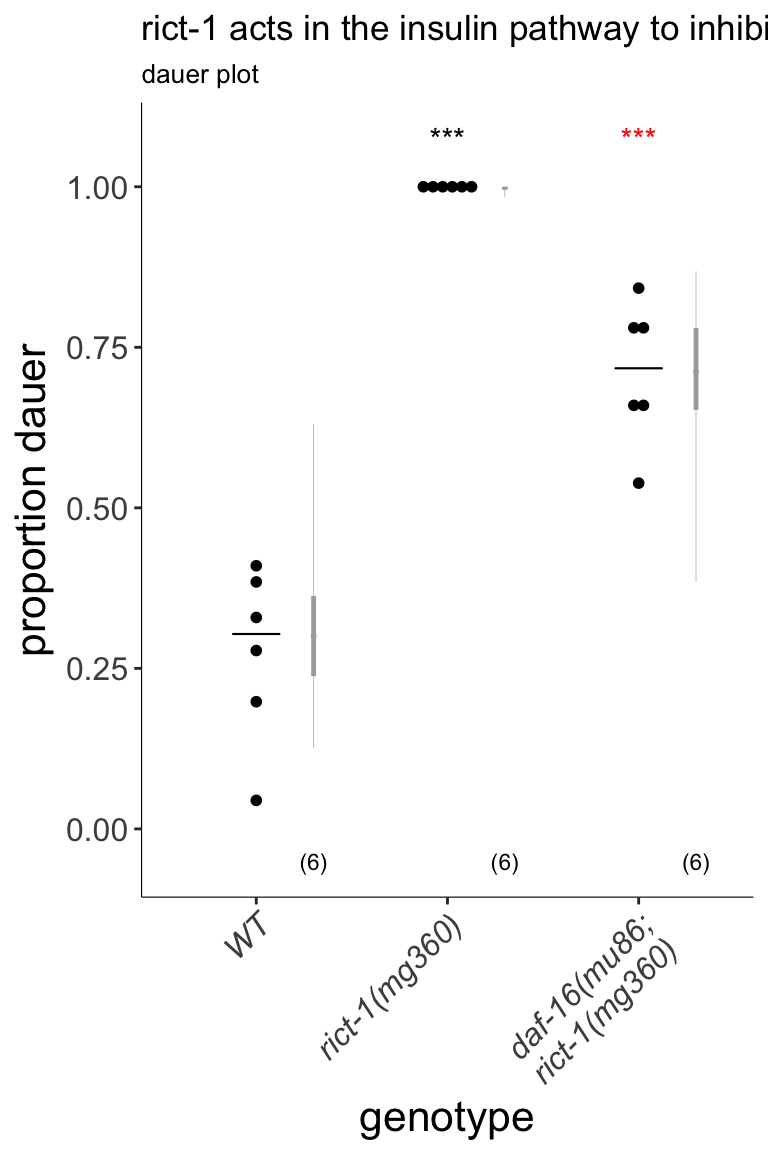
\includegraphics{Figure_2_files/figure-latex/plot daf-16-1.pdf}

 \textbf{Figure S1E} Mutations in rict-1 modulate dauer formation via
downregulation of neuroendocrine signaling. \emph{daf-16} mutations
partially suppress the dauer formation phenotype of \emph{rict-1}
mutants. Dauers formed by animals of the indicated genotypes at 27°C.
Each dot indicates the proportion of dauers formed in a single assay.
Horizontal bar indicates median. Light gray thin and thick vertical bars
at right indicate Bayesian 95\% and 75\% credible intervals,
respectively. Numbers in parentheses below indicate the number of
independent experiments with at least 26 animals each. {\texttt{***}} -
different from wild-type at P\textless{}0.001, {\texttt{***}} -
different from rict-1(mg360) at P\textless{}0.001 (ANOVA with Tukey-type
multivariate-t post-hoc adjustments). P-values of differences in means
relative to wild-type and corresponding mutant animals are indicated in
black and red, respectively.

\begin{Shaded}
\begin{Highlighting}[]
\KeywordTok{library}\NormalTok{(sjPlot)}
\KeywordTok{sjt.lm}\NormalTok{(lm, }\DataTypeTok{depvar.labels =} \StringTok{"proportion of dauers"}\NormalTok{, }\DataTypeTok{show.se =} \OtherTok{TRUE}\NormalTok{, }\DataTypeTok{show.fstat =} \OtherTok{TRUE}\NormalTok{)}
\end{Highlighting}
\end{Shaded}

~

~

proportion of dauers

~

~

B

CI

std. Error

p

(Intercept)

~

0.27

0.19~--~0.36

0.04

\textless{}.001

genotype

rict-1(mg360)

~

0.73

0.60~--~0.85

0.06

\textless{}.001

rict-1;daf-16

~

0.44

0.31~--~0.56

0.06

\textless{}.001

Observations

~

18

R2 / adj. R2

~

.912 / .901

F-statistics

~

77.980***

\begin{Shaded}
\begin{Highlighting}[]
\NormalTok{knitr}\OperatorTok{::}\KeywordTok{kable}\NormalTok{(contrasts, }\DataTypeTok{caption=}\StringTok{"Pairwise comparisons from ANOVA (Tukey)"}\NormalTok{)}
\end{Highlighting}
\end{Shaded}

\begin{longtable}[]{@{}lrrrrrl@{}}
\caption{Pairwise comparisons from ANOVA (Tukey)}\tabularnewline
\toprule
contrast & estimate & SE & df & t.ratio & p.value &
prange\tabularnewline
\midrule
\endfirsthead
\toprule
contrast & estimate & SE & df & t.ratio & p.value &
prange\tabularnewline
\midrule
\endhead
N2 - rict-1(mg360) & -0.7259908 & 0.0585246 & 15 & -12.404877 &
0.0000000 & ***\tabularnewline
N2 - rict-1;daf-16 & -0.4360625 & 0.0585246 & 15 & -7.450922 & 0.0000050
& ***\tabularnewline
rict-1(mg360) - rict-1;daf-16 & 0.2899283 & 0.0585246 & 15 & 4.953954 &
0.0004179 & ***\tabularnewline
\bottomrule
\end{longtable}

\begin{Shaded}
\begin{Highlighting}[]
\NormalTok{knitr}\OperatorTok{::}\KeywordTok{kable}\NormalTok{(mixed[,}\KeywordTok{c}\NormalTok{(}\DecValTok{6}\NormalTok{,}\DecValTok{1}\OperatorTok{:}\DecValTok{5}\NormalTok{)], }\DataTypeTok{caption =} \StringTok{"Bayesian credible intervals"}\NormalTok{)}
\end{Highlighting}
\end{Shaded}

\begin{longtable}[]{@{}lrrrrr@{}}
\caption{Bayesian credible intervals}\tabularnewline
\toprule
genotype & mean & lower.CL & upper.CL & lower.25 &
upper.75\tabularnewline
\midrule
\endfirsthead
\toprule
genotype & mean & lower.CL & upper.CL & lower.25 &
upper.75\tabularnewline
\midrule
\endhead
N2 & 0.3009765 & 0.1261611 & 0.6307367 & 0.2378515 &
0.3625799\tabularnewline
rict-1(mg360) & 0.9979362 & 0.9835708 & 0.9998078 & 0.9956347 &
0.9989622\tabularnewline
rict-1;daf-16 & 0.7126570 & 0.3850782 & 0.8685749 & 0.6525277 &
0.7801805\tabularnewline
\bottomrule
\end{longtable}


\end{document}
